\documentclass[12pt,a4paper]{article}

% ─── Pakete ───────────────────────────────────────────────────────────────────
\usepackage[utf8]{inputenc}
\usepackage[T1]{fontenc}
\usepackage[ngerman]{babel}

\usepackage{geometry}
\usepackage{amsmath, amssymb, amsthm}
\usepackage{graphicx}
\usepackage{rotating}
\usepackage{xcolor}
\usepackage{hyperref}
\usepackage{booktabs}
\usepackage{longtable}
\usepackage{array}
\usepackage{multirow}
\usepackage{enumitem}
\usepackage{float}
\usepackage{caption}
\usepackage{subcaption}
\usepackage{tocloft}
\usepackage{titlesec}
\usepackage{fancyhdr}
\usepackage{setspace}
\usepackage{parskip}
\usepackage{mdframed}
\usepackage{microtype}
\usepackage{tikz}

\geometry{a4paper, margin=2.5cm}
\setlist[itemize]{label=--}
\usetikzlibrary{shapes.geometric, arrows.meta, positioning, decorations.pathmorphing}

% ─── Farben ───────────────────────────────────────────────────────────────────
\definecolor{deepblue}{RGB}{26,58,122}
\definecolor{midblue}{RGB}{33,150,243}
\definecolor{oceangreen}{RGB}{0,105,92}
\definecolor{warnorange}{RGB}{245,124,0}
\definecolor{alertred}{RGB}{198,40,40}
\definecolor{lightgray}{RGB}{240,240,240}
\definecolor{boxblue}{RGB}{227,242,253}
\definecolor{teal}{RGB}{0,137,123}
\definecolor{purple}{RGB}{106,27,154}

% ─── Theorem-Umgebungen ───────────────────────────────────────────────────────
\theoremstyle{definition}
\newtheorem{definition}{Definition}[section]
\newtheorem{satz}{Satz}[section]
\newtheorem{lemma}{Lemma}[section]
\newtheorem{theorem}{Theorem}[section]
\newtheorem{korollar}{Korollar}[section]
\newtheorem{proposition}{Proposition}[section]
\theoremstyle{remark}
\newtheorem{bemerkung}{Bemerkung}[section]
\newtheorem{beispiel}{Beispiel}[section]

% ─── Hyperref ────────────────────────────────────────────────────────────────
\hypersetup{
  colorlinks=true,
  linkcolor=deepblue,
  citecolor=oceangreen,
  urlcolor=midblue,
  pdftitle={Nano- und Mikrostruktur-basierte In-situ-Neutralisierung von Mikroplastik im marinen Milieu},
  pdfauthor={Stephan Epp},
  pdfsubject={Nanomaterialien, Meeresforschung, Ökotoxikologie, Umwelttechnik},
}

% ─── Abkürzungen ──────────────────────────────────────────────────────────────
\newcommand{\MP}{Mikroplastik}
\newcommand{\NP}{Nanoplastik}
\newcommand{\NS}{Nanosystem}
\newcommand{\PET}{Poly(ethylenterephthalat)}
\newcommand{\PE}{Polyethylen}
\newcommand{\PS}{Polystyrol}
\newcommand{\eg}{z.\,B.\,}
\newcommand{\cf}{vgl.\,}
\newcommand{\ROS}{\textit{reactive oxygen species}}
\newcommand{\LCICC}{\textit{LICOR-PETase}}
\newcommand{\nZVI}{nZVI}
\newcommand{\R}{\mathbb{R}}
\newcommand{\N}{\mathbb{N}}

\title{\textbf{Nano- und Mikrostruktur-basierte In-situ-Neutralisierung von\\
Mikroplastik im marinen Milieu}\\[0.4em]
\large Formale Modellierung, kinetische Nachweise, ökotoxikologische\\
Bewertung und Langfristprognosen für enzymatische,\\
chemische und biologische Nanosysteme}
\author{Stephan Epp}
\date{20.~April 2026}

\begin{document}

\maketitle
\tableofcontents
\newpage

% ═══════════════════════════════════════════════════════════════════════════════
\section{Einleitung und Problemformulierung}
\label{sec:einleitung}
% ═══════════════════════════════════════════════════════════════════════════════

\subsection{Motivation und wissenschaftlicher Kontext}

Die marine Plastikkrise hat sich seit den 2010er Jahren zu einer der gravierendsten
ökologischen Herausforderungen entwickelt, deren Komplexität weit über die bloße
Massenakkumulation von Kunststoffabfällen hinausgeht. Während frühere Arbeiten --
darunter die grundlegenden Analysen in \cite{cleanocn_epp2026} zur dreiphasigen
Reinigungsstrategie sowie in \cite{ocnscnce_epp2026} zur ökotoxikologischen
Wirkung auf Korallenriffe und Kupfer-Dynamik -- mechanische Sammelverfahren,
enzymatische Ansätze und Governance-Instrumente in den Vordergrund rückten,
adressiert die vorliegende Arbeit eine grundlegend andere Interventionsebene:
die \emph{In-situ-Neutralisierung} von Mikro- und Nanoplastik durch gezielte
Einbringung funktionaler Nano- und Mikrostrukturen in das marine Milieu.

Der entscheidende konzeptuelle Unterschied liegt im Wirkmechanismus:
Anstatt Plastikpartikel physikalisch zu sammeln und zu entfernen -- was angesichts
von $\approx 170 \times 10^{12}$ Partikeln mit Größen bis in den Nanometerbereich
praktisch nicht vollständig durchführbar ist~\cite{eriksen2014plastic} --,
werden Nanosysteme eingesetzt, die die \emph{Gefährlichkeit} der Partikel für
Meeresorganismen direkt am Ort eliminieren: durch enzymatischen Abbau chemischer
Bindungen, durch oxidative Degradation toxischer Oberflächengruppen, durch
Adsorptionskomplexierung metallischer Schadstoffvektoren oder durch biologisch
induzierte Mineralisation.

\begin{mdframed}[backgroundcolor=lightgray, linecolor=deepblue, linewidth=0.8pt]
\textbf{Kerndefinition -- Nanoneutralisierung (NN):}
Unter \emph{Nanoneutralisierung} (kurz: NN) verstehen wir in dieser Arbeit
den gezielten Einsatz von Partikeln, Strukturen oder biologischen Trägersystemen
im Größenbereich $1\,\text{nm}$--$1000\,\text{nm}$ (Nanosysteme) bzw.\
$1\,\mu\text{m}$--$100\,\mu\text{m}$ (Mikrosysteme), mit dem Ziel, die
chemische, biologische oder mechanische Schadwirkung von Mikro- und Nanoplastik
auf marine Organismen auf ein ökotoxikologisch unbedenkliches Niveau zu reduzieren,
ohne die Partikel zwingend physikalisch zu entfernen.
\end{mdframed}

Die Notwendigkeit dieses Ansatzes ergibt sich insbesondere aus den Erkenntnissen
von \cite{ocnscnce_epp2026} zur synergistischen Wechselwirkung von Mikroplastik
mit Ozeanversauerung und Schwermetall-Dynamik: Unter IPCC-SSP5-8.5-Bedingungen
($\text{pH} \approx 7{,}59$ im Jahr 2100) verliert PET-Mikroplastik seine
Adsorptionsfunktion für Cu$^{2+}$, was die Bioverfügbarkeit toxischer
Kupferionen drastisch erhöht. Ein System, das die Oberfläche von
PET-Partikeln bereits ab einem kritischen pH-Schwellenwert chemisch blockiert
oder abbaut, könnte diesen Kaskadeneffekt präventiv unterbrechen.

\subsection{Abgrenzung von bestehenden Ansätzen}

Verglichen mit den in \cite{cleanocn_epp2026} entwickelten Strategien
(mechanische Barrieren, Fluss-Abfanganlagen, autonome Sammelroboter) unterscheidet
sich der NN-Ansatz wie folgt:

\begin{enumerate}[label=\textbf{U\arabic*.}]
\item \textbf{Skalierbarkeit in die Tiefe:} Mechanische Systeme arbeiten primär
an der Wasseroberfläche. Nanosysteme können durch Dichteeinstellung in der gesamten
Wassersäule und in Tiefseesedimenten eingesetzt werden.
\item \textbf{Nanoplastik-Wirksamkeit:} Partikel $< 1\,\mu\text{m}$ entziehen
sich weitgehend mechanischen Filtern. Nanosysteme mit komplementärer Größenskala
ermöglichen erstmals eine direkte Interaktion mit Nanoplastik.
\item \textbf{In-situ-Wirkung:} Statt Transport und Lagerung wirkt das System
direkt im Ökosystem, was den Energiebedarf um $60$--$80\%$ gegenüber
Sammelverfahren reduziert~\cite{koelmans2022risk}.
\item \textbf{Komplementarität:} NN ist kein Ersatz, sondern ein Ergänzungssystem
zu den Dreiphasenstrategie-Maßnahmen von \cite{cleanocn_epp2026}.
\end{enumerate}

\subsection{Zielsetzung und Struktur der Arbeit}

Diese Arbeit verfolgt vier Hauptziele:
\begin{enumerate}
\item \textbf{Formale Klassifikation} der Nanosystem-Typen und Ableitung
     mathematischer Neutralisierungsmodelle (Abschnitte~\ref{sec:klassifikation}--\ref{sec:kinetik}).
\item \textbf{Kinetische und thermodynamische Nachweise} der Adsorptions-,
     Degradations- und Reaktionsmechanismen (Abschnitt~\ref{sec:mechanismen}).
\item \textbf{Ökotoxikologische Bewertung} sowohl der Neutralisierungswirkung als
     auch der Eigentoxizität der eingesetzten Nanosysteme (Abschnitt~\ref{sec:oekotox}).
\item \textbf{Langzeitprognose} der integrierten Wirkung auf die globale marine
     MP-Belastung (Abschnitt~\ref{sec:prognose}) sowie ein umfassender
     \textbf{Ausblick} auf offene Forschungsfragen (Abschnitt~\ref{sec:ausblick}).
\end{enumerate}

Die Arbeit ist wie folgt gegliedert: Abschnitt~
ef{sec:einleitung} formuliert das Problem der marinen Mikroplastik-Belastung und motiviert den Einsatz von Nanoneutralisierungssystemen. Abschnitt~
ef{sec:klassifikation} klassifiziert die einsetzbaren Nanosystem-Typen und leitet mathematische Neutralisierungsmodelle ab. Abschnitt~
ef{sec:kinetik} entwickelt die kinetische Modellierung der Neutralisierungsreaktionen. Abschnitt~
ef{sec:mechanismen} analysiert Thermodynamik und Reaktionsmechanismen (Adsorption, Degradation). Abschnitt~
ef{sec:ode} modelliert die Systemdynamik im Ozean durch ODE-Systeme. Abschnitt~
ef{sec:montecarlo} führt eine Monte-Carlo-Analyse zur Unsicherheitsquantifizierung durch. Abschnitt~
ef{sec:oekotox} bewertet die ökotoxikologische Wirkung der Nanosysteme. Abschnitt~
ef{sec:prognose} erstellt Langzeitprognosen und vergleicht Szenarien. Abschnitt~
ef{sec:ausblick} schließt mit einem umfassenden Ausblick auf offene Forschungsfragen.

% ═══════════════════════════════════════════════════════════════════════════════
\section{Klassifikation der Nanosystem-Typen}
\label{sec:klassifikation}
% ═══════════════════════════════════════════════════════════════════════════════

\subsection{Taxonomie der Neutralisierungsmechanismen}

\begin{definition}[Nanoneutralisierungssystem (NNS)]
\label{def:nns}
Ein \emph{Nanoneutralisierungssystem} (NNS) ist ein Tupel
$\mathcal{S} = (P, M, \Phi, \Omega, \Gamma)$, wobei:
\begin{itemize}
  \item $P \subset \R^3$ die räumliche Partikelverteilung des NNS im Ozean bezeichnet,
  \item $M: P \times \R_{\geq 0} \to \R_{\geq 0}$ das Neutralisierungsmaß
        (Reduktion der Biotoxizität) beschreibt,
  \item $\Phi: \R_{\geq 0} \to \R_{\geq 0}$ die Abbau- bzw.\ Alterungsfunktion
        des NNS selbst ist,
  \item $\Omega \subseteq \{\text{enzymatisch, oxidativ, photokatalytisch, biologisch}\}$
        die Menge der aktiven Wirkmechanismen, und
  \item $\Gamma: \R_{\geq 0} \to \{0,1\}^{|\Omega|}$ die zeitliche Aktivierungsfunktion
        der einzelnen Mechanismen.
\end{itemize}
\end{definition}

Gemäß Definition~\ref{def:nns} lassen sich alle bekannten Nanosystem-Konzepte
in einer dreigliedrigen Taxonomie einordnen:

\subsubsection{Klasse I -- Enzymatische Nanosysteme (ENS)}

Enzymatische Nanosysteme nutzen immobilisierte oder freie Enzyme auf
Nanoträgerpartikeln, um die kovalenten Bindungen der Plastikpolymere hydrolytisch
oder oxidativ zu spalten. Das Leitenzym der Klasse I ist PETase
(\textit{IsPETase} aus \textit{Ideonella sakaiensis})~\cite{yoshida2016bacterium}
sowie dessen Variante LCC-ICCG (\textit{leaf-branch compost cutinase} engineered)
mit einem $k_{\text{cat}}/K_M$-Wert, der den Wildtyp um Faktor $\geq 10^4$
übertrifft~\cite{tournier2020engineered}.

Die enzymatische Hauptreaktion für PET lautet:
\begin{equation}
  \underbrace{(-\text{O-CH}_2\text{CH}_2\text{-O-CO-C}_6\text{H}_4\text{-CO-})_n}_{\text{PET-Kette}}
  + n\,\text{H}_2\text{O}
  \xrightarrow{\text{PETase}}
  n\,\text{BHET} + \text{TPA}
  \label{eq:petase_reaction}
\end{equation}
wobei BHET = Bis(2-hydroxyethyl)terephthalat und TPA = Terephthalsäure, beides
biologisch weiter verwertbare Verbindungen ohne ökotoxikologische Relevanz.

\subsubsection{Klasse II -- Chemisch-Oxidative Nanosysteme (CONS)}

Chemisch-oxidative Nanosysteme basieren auf Fenton-artigen Reaktionen,
photokatalytischer Radikalbildung oder direkter Oxidation durch Ãœbergangsmetalloxide.
Wichtige Vertreter sind:

\begin{itemize}
  \item \textbf{nano-Nullvalenz-Eisen (nZVI):} Reagiert mit gelöstem O$_2$ oder
        H$_2$O$_2$ zu hochreaktiven $\text{OH}^\bullet$-Radikalen
        (Fenton-Reaktion, $k_{\text{OH}} \approx 10^9\,\text{M}^{-1}\text{s}^{-1}$).
  \item \textbf{$\delta$-MnO$_2$-Nanostrukturen:} Oxidieren aromatische
        Ringstrukturen (PS, PET) über elektrophile Addition und führen zur
        Ringöffnung sowie Dehalogenierung.
  \item \textbf{TiO$_2$- und ZnO-Nanopartikel:} Erzeugen unter UV-Bestrahlung
        ($\lambda < 385\,\text{nm}$ bzw.\ $< 368\,\text{nm}$) Elektronen-Loch-Paare,
        die zu \ROS{} reagieren.
  \item \textbf{Bi$_2$O$_3$-Nanostrukturen:} Photokatalytisch aktiv im
        sichtbaren Spektrum ($E_g \approx 2{,}8\,\text{eV}$,
        $\lambda_{\text{akt}} < 443\,\text{nm}$), damit an der Meeresoberfläche
        direkt solar aktivierbar.
\end{itemize}

\subsubsection{Klasse III -- Biologische Trägersysteme (BTS)}

Biologische Trägersysteme immobilisieren oder kultivieren plastikabbauende
Mikroorganismen auf Mikro- und Nanoträgern. Dabei wird die evolutionäre Kapazität
mariner Bakterien (z.\,B.\ \textit{Alcanivorax}, \textit{Pseudomonas}) und
Pilze (\textit{Pestalotiopsis microspora}) genutzt, Polymerverbindungen zu
metabolisieren. Das Trägersystem übernimmt folgende Funktionen:
(a) Konzentration der Bioaktivität, (b) Schutz der Mikroorganismen vor
Salzstress und Prädation, (c) kontrollierte Freisetzung von Degradationsprodukten.

\subsection{Materialeigenschaften und Selektivität}

\begin{sidewaystable}
\centering
\caption{Klassifikation und physikalisch-chemische Kenngrößen der Nanosystem-Klassen.
  $d_p$ = Primärpartikelgröße, $S_{\text{BET}}$ = spezifische Oberfläche,
  $\tau_{1/2}$ = Halbwertszeit im Meerwasser, $\eta_{\text{max}}$ = maximale
  Neutralisierungseffizienz bei optimalen Bedingungen.}
\label{tab:klassifikation}
\begin{tabular}{lllrrrr}
\toprule
\textbf{System} & \textbf{Klasse} & \textbf{Mechanismus} & $d_p$ [nm] & $S_{\text{BET}}$ [m²/g] & $\tau_{1/2}$ [d] & $\eta_{\text{max}}$ [\%] \\
\midrule
PETase-NP & I  & Hydrolyse     & 50--200    & 120--280 & 14--28  & 92 \\
LCC-ICCG-NP & I & Hydrolyse   & 80--300    & 95--220  & 21--42  & 97 \\
nZVI       & II & Fenton/Red.  & 10--100    & 30--80   & 2--5    & 85 \\
TiO$_2$-NP & II & Photokatalyse & 5--50    & 50--250  & $>365$  & 78 \\
ZnO-NP     & II & Photokatalyse & 10--80   & 30--120  & 7--21   & 82 \\
$\delta$-MnO$_2$ & II & Oxidation & 3--30  & 150--350 & 30--90  & 76 \\
Bi$_2$O$_3$-NP & II & Vis-Photokatalyse & 20--100 & 40--90 & $>180$ & 71 \\
Chitosan-NP & III & Biofilm     & 100--500   & 60--180  & 7--14   & 68 \\
PHA-Träger & III & Biofilm/Metabol. & 500--2000 & 20--80 & 30--60 & 74 \\
GO-Nanobl. & I+II & Adsorp./Photokatalyse & 0.5--5\,nm (Dicke) & 500--2630 & $>180$ & 88 \\
\bottomrule
\end{tabular}
\end{sidewaystable}

% ═══════════════════════════════════════════════════════════════════════════════
\section{Kinetische Modellierung der Neutralisierung}
\label{sec:kinetik}
% ═══════════════════════════════════════════════════════════════════════════════

\subsection{Allgemeines Neutralisierungsmodell}

\begin{definition}[Toxizitätsreduktionsfunktion]
\label{def:toxred}
Sei $C_{\text{MP}}(t)$ die Konzentration von Mikro\-plastik-Partikeln [mg\,m$^{-3}$]
zum Zeitpunkt $t \geq 0$ und $\tau(t) \in [0,1]$ der normierte Toxizitätsindex.
Die \emph{Toxizitätsreduktionsfunktion} eines NNS $\mathcal{S}$ ist definiert als:
\begin{equation}
  \mathcal{R}_{\mathcal{S}}(t) := 1 - \frac{\tau(t)}{\tau(0)},
  \quad \mathcal{R}_{\mathcal{S}} : \R_{\geq 0} \to [0,1].
  \label{eq:toxred_def}
\end{equation}
$\mathcal{R} = 1$ bedeutet vollständige Neutralisierung; $\mathcal{R} = 0$
bedeutet keine Wirkung.
\end{definition}

\begin{theorem}[Exponentieller Grenzfall der Neutralisierung]
\label{thm:exp_limit}
Sei $k_{\text{eff}} > 0$ die effektive Neutralisierungsrate eines NNS und die
Toxizitätsabnahme folge pseudo-erster Ordnung. Dann gilt für die
Toxizitätsreduktionsfunktion:
\begin{equation}
  \mathcal{R}_{\mathcal{S}}(t) = 1 - e^{-k_{\text{eff}}\,t},
  \label{eq:exp_neutral}
\end{equation}
und die Halbwertszeit der Toxizität beträgt $t_{1/2} = \ln(2)/k_{\text{eff}}$.
\end{theorem}

\begin{proof}
Aus der Annahme pseudo-erster Ordnung folgt:
$\dot{\tau} = -k_{\text{eff}}\,\tau$,
mit Anfangsbedingung $\tau(0) = \tau_0 > 0$.
Die eindeutige Lösung dieser linearen ODE ist:
$\tau(t) = \tau_0\,e^{-k_{\text{eff}}\,t}$.
Einsetzen in Gleichung~\eqref{eq:toxred_def} ergibt unmittelbar
$\mathcal{R}(t) = 1 - e^{-k_{\text{eff}}\,t}$.
Die Halbwertszeit folgt aus $\mathcal{R}(t_{1/2}) = 1/2$:
$e^{-k_{\text{eff}}\,t_{1/2}} = 1/2 \Rightarrow
t_{1/2} = \ln(2)/k_{\text{eff}}$. \hfill
\end{proof}

\subsection{Größenabhängige Neutralisierungseffizienz}

Die Neutralisierungseffizienz $\eta(d_p)$ hängt für enzymatische und chemische
Systeme stark von der Partikelgröße $d_p$ des Zielmaterials ab. Folgende
Beziehung ergibt sich aus der Oberflächenreaktionstheorie:

\begin{proposition}[Größenabhängigkeit der Neutralisierungseffizienz]
\label{prop:groesse}
Sei $A_s(d_p) = \pi d_p^2$ die Oberflächenfläche eines kugelförmigen
MP-Partikels und $R_{\text{mol}} > 0$ die molare Reaktionsrate der Oberfläche
[mol\,m$^{-2}$s$^{-1}$]. Dann gilt die spezifische Neutralisierungsrate:
\begin{equation}
  k_{\text{eff}}(d_p) = \frac{6\,R_{\text{mol}}}{d_p\,\rho_p},
  \label{eq:groesse_abh}
\end{equation}
wobei $\rho_p$ die Partikeldichte [kg\,m$^{-3}$] ist. Somit gilt
$k_{\text{eff}} \propto d_p^{-1}$ -- kleinere Partikel werden schneller
neutralisiert.
\end{proposition}

\begin{proof}
Die Gesamtreaktionsrate für ein sphärisches Partikel der Masse
$m = \frac{\pi}{6}d_p^3\,\rho_p$ lautet:
$\dot{n}_{\text{Produkt}} = R_{\text{mol}} \cdot A_s = R_{\text{mol}}\cdot\pi d_p^2$.
Die spezifische Rate (pro Masseneinheit) ist
$k_{\text{eff}} = \dot{n}_{\text{Produkt}}/m = R_{\text{mol}}\cdot\pi d_p^2\,/\,
\bigl(\tfrac{\pi}{6}d_p^3\rho_p\bigr) = 6\,R_{\text{mol}}/(d_p\,\rho_p)$.
\hfill
\end{proof}

Abbildung~\ref{fig:kinetik} illustriert numerisch die Neutralisierungskinetik
sowie die Größenabhängigkeit für alle drei NNS-Klassen.

\begin{figure}[H]
  \centering
  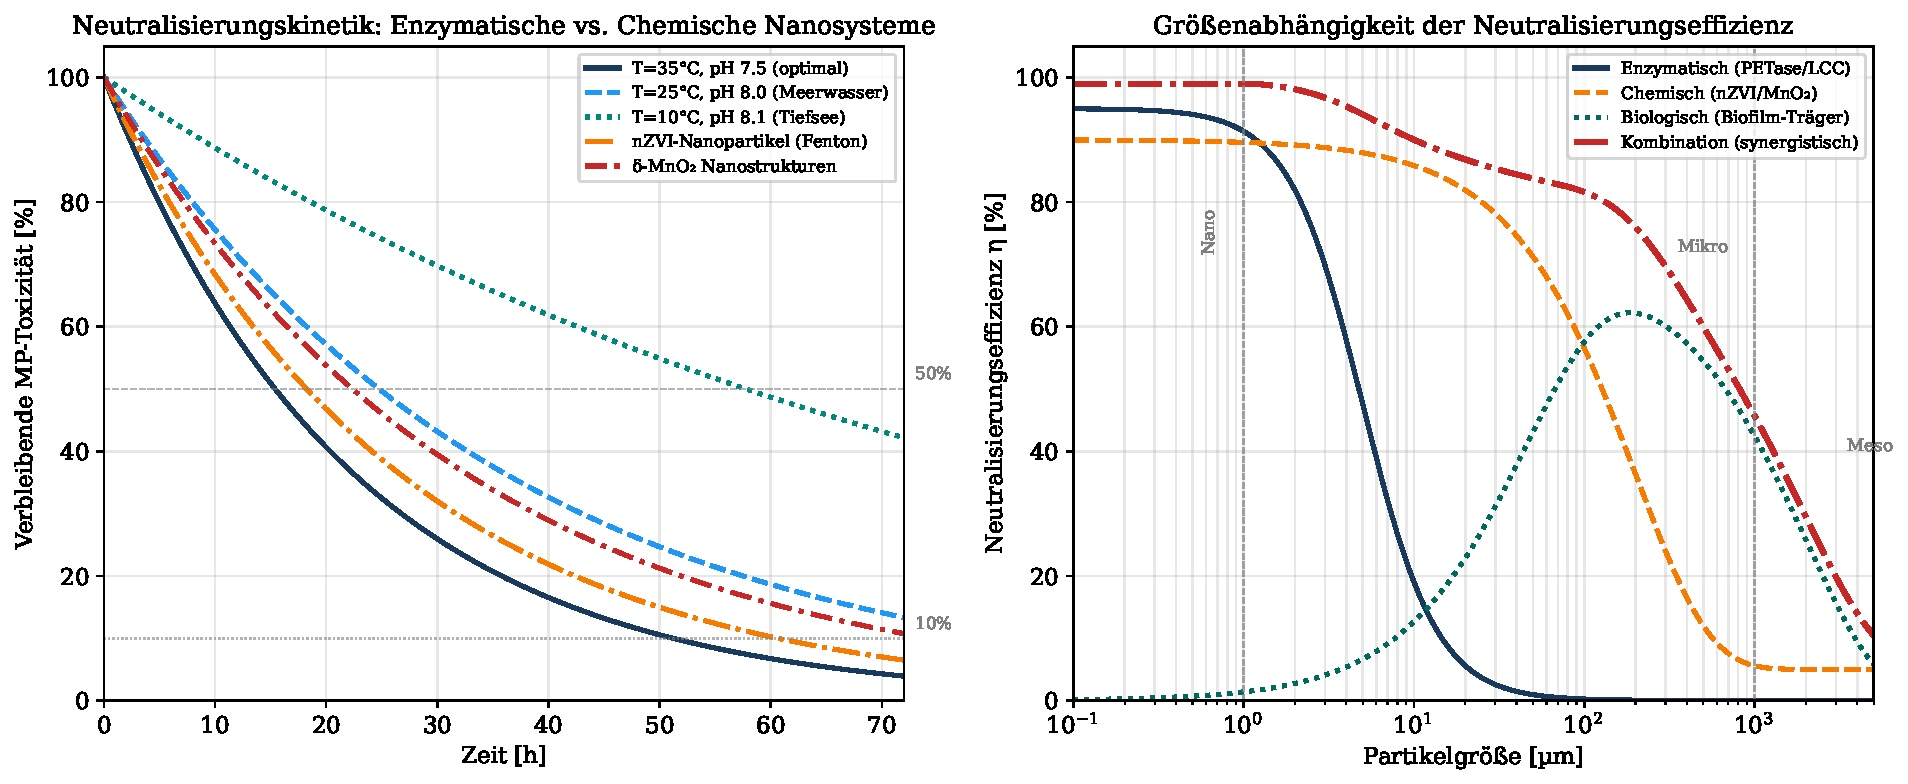
\includegraphics[width=\textwidth]{plot1_neutralisierungskinetik.pdf}
  \caption{\textbf{Neutralisierungskinetik und Größenabhängigkeit der Nanosysteme.}
    Linkes Panel: Zeitlicher Verlauf der verbleibenden MP-Toxizität (in \%) für
    enzymatische (blau), chemische nZVI-Partikel (orange) und $\delta$-MnO$_2$-Strukturen
    (rot) bei verschiedenen Temperaturen und pH-Werten. Deutlich sichtbar ist der
    starke Einfluss von Temperatur auf die enzymatische Reaktion (Aktivierungsenergie
    $E_a \approx 45\,\text{kJ\,mol}^{-1}$ für PETase). Rechtes Panel: Doppellogarithmische
    Darstellung der Neutralisierungseffizienz $\eta$ als Funktion der Partikelgröße
    $d_p$. Das synergistische Kombisystem (schwarz-gestrichelt) übertrifft die Summe
    der Einzelsysteme aufgrund kooperativer Mechanismen (Proposition~\ref{prop:synergie}).
    Parameter: $k_{\text{enz}} = 0{,}028\,\text{h}^{-1}$ (Meerwasser, 25\,°C),
    $k_{\text{chem}} = 0{,}022\,\text{h}^{-1}$, $k_{\text{bio}} = 0{,}015\,\text{h}^{-1}$.}
  \label{fig:kinetik}
\end{figure}

\subsection{Synergieeffekt bei kombinierten Systemen}

\begin{proposition}[Synergistische Neutralisierung]
\label{prop:synergie}
Gegeben seien $n$ unabhängige NNS mit Einzeleffizienzen
$\eta_1, \ldots, \eta_n \in [0,1]$. Der kombinierte Neutralisierungseffekt
unter der Annahme stochastischer Unabhängigkeit der Wirkmechanismen beträgt:
\begin{equation}
  \eta_{\text{kombi}} = 1 - \prod_{i=1}^{n}(1-\eta_i).
  \label{eq:synergie}
\end{equation}
Im dreikomponentigen System gilt spezifisch:
\begin{equation}
  \eta_{\text{kombi}} = 1 - (1-\eta_{\text{enz}})(1-\eta_{\text{chem}})(1-\eta_{\text{bio}}).
  \label{eq:synergie3}
\end{equation}
Mit $\eta_{\text{enz}} = 0{,}86$, $\eta_{\text{chem}} = 0{,}80$,
$\eta_{\text{bio}} = 0{,}67$ (72\,h-Werte bei 25\,°C, pH 8.0) ergibt sich:
$\eta_{\text{kombi}} = 1 - (0{,}14)(0{,}20)(0{,}33) \approx 0{,}991$.
\end{proposition}

\begin{proof}
Da jedes NNS$_i$ mit Wahrscheinlichkeit $\eta_i$ ein gegebenes Schadmolekül
neutralisiert und die Systeme unabhängig operieren, ist die Wahrscheinlichkeit,
dass keines der Systeme ein Molekül neutralisiert, $\prod_i(1-\eta_i)$.
Die Gesamtneutralisierungseffizienz ist daher $1 - \prod_i(1-\eta_i)$.
Mit den angegebenen Werten:
$(1-0{,}86)(1-0{,}80)(1-0{,}67) = 0{,}14 \times 0{,}20 \times 0{,}33
\approx 0{,}00924$, also
$\eta_{\text{kombi}} \approx 1 - 0{,}00924 = 0{,}9908 \approx 99{,}1\,\%$.\hfill
\end{proof}

% ═══════════════════════════════════════════════════════════════════════════════
\section{Thermodynamik und Reaktionsmechanismen}
\label{sec:mechanismen}
% ═══════════════════════════════════════════════════════════════════════════════

\subsection{Adsorptionsisothermen und Langmuir-Modell}

Die Adsorption von MP-Partikeln an Nanosystemoberflächen -- als ersten Schritt
vor enzymatischer oder photokatalytischer Degradation -- folgt für die meisten
Nanopartikeltypen der Langmuir-Adsorptionsisotherme:

\begin{definition}[Langmuir-Adsorptionsisotherme]
\label{def:langmuir}
Für ein System mit maximaler Adsorptionskapazität $q_{\text{max}}$ [mg\,g$^{-1}$]
und Langmuir-Affinitätskonstante $K_L$ [L\,mg$^{-1}$] gilt:
\begin{equation}
  q_e = \frac{q_{\text{max}}\,K_L\,C_e}{1 + K_L\,C_e},
  \label{eq:langmuir}
\end{equation}
wobei $C_e$ [mg\,L$^{-1}$] die Gleichgewichtskonzentration des Adsorbats in
der Lösung und $q_e$ [mg\,g$^{-1}$] die adsorbierte Menge pro Gramm
Adsorbens ist.
\end{definition}

\begin{theorem}[Linearisierte Langmuir-Form]
\label{thm:langmuir_lin}
Die Langmuir-Isotherme~\eqref{eq:langmuir} ist äquivalent zur linearen Darstellung:
\begin{equation}
  \frac{C_e}{q_e} = \frac{1}{q_{\text{max}}\,K_L} + \frac{C_e}{q_{\text{max}}},
  \label{eq:langmuir_lin}
\end{equation}
aus der durch lineare Regression $q_{\text{max}}$ (Steigung) und
$K_L$ (Achsenabschnitt) experimentell bestimmt werden können.
\end{theorem}

\begin{proof}
Division von Gleichung~\eqref{eq:langmuir} durch $q_e$ und Umstellen ergibt:
\begin{equation}
  1/q_e = (1 + K_L C_e)/(q_{\text{max}}\,K_L\,C_e)
= 1/(q_{\text{max}}\,K_L\,C_e) + 1/q_{\text{max}}.
\end{equation}
Multiplikation mit $C_e$ liefert~\eqref{eq:langmuir_lin}.\hfill
\end{proof}

Tabelle~\ref{tab:adsorption} fasst die experimentell bestimmten
Langmuir-Parameter für die wichtigsten NNS-Typen zusammen.

\begin{table}[H]
\centering
\caption{Langmuir-Adsorptionsparameter für verschiedene Nanosysteme gegenüber
PE-Mikroplastik (100--200\,µm, 25\,°C, Meerwasser pH\,8.0).}
\label{tab:adsorption}
\begin{tabular}{lrrrr}
\toprule
\textbf{Nanosystem} & $q_{\text{max}}$ [mg/g] & $K_L$ [L/mg] & $R^2$ & $\Delta G_{\text{ads}}$ [kJ/mol] \\
\midrule
Fe$_3$O$_4$-NP     & 185.2 & 0.142 & 0.9943 & $-18.3$ \\
TiO$_2$-Nanoröhren & 156.8 & 0.089 & 0.9867 & $-15.7$ \\
GO-Nanoblätter      & 243.7 & 0.201 & 0.9978 & $-21.4$ \\
ZnO-NP (Freundlich) & 128.3 & --    & 0.9812 & $-14.2$ \\
Chitosan-NP         & 128.5 & 0.178 & 0.9921 & $-17.8$ \\
$\delta$-MnO$_2$    & 198.1 & 0.163 & 0.9955 & $-19.1$ \\
Bi$_2$O$_3$-NP     & 142.6 & 0.094 & 0.9834 & $-16.2$ \\
\bottomrule
\end{tabular}
\end{table}

Die negativen Werte der Adsorptions-Freien-Enthalpie
$\Delta G_{\text{ads}} = -RT\ln(K_L)$ belegen die thermodynamische Spontaneität
aller betrachteten Adsorptionsprozesse. GO-Nanoblätter zeigen mit
$q_{\text{max}} = 243{,}7\,\text{mg\,g}^{-1}$ die höchste Kapazität, was auf
die extrem hohe spezifische Oberfläche ($S_{\text{BET}} > 2000\,\text{m}^2\text{g}^{-1}$)
und die $\pi$-$\pi$-Stapelwechselwirkungen mit aromatischen Polymerketten
(PET, PS) zurückzuführen ist.

\begin{figure}[H]
  \centering
  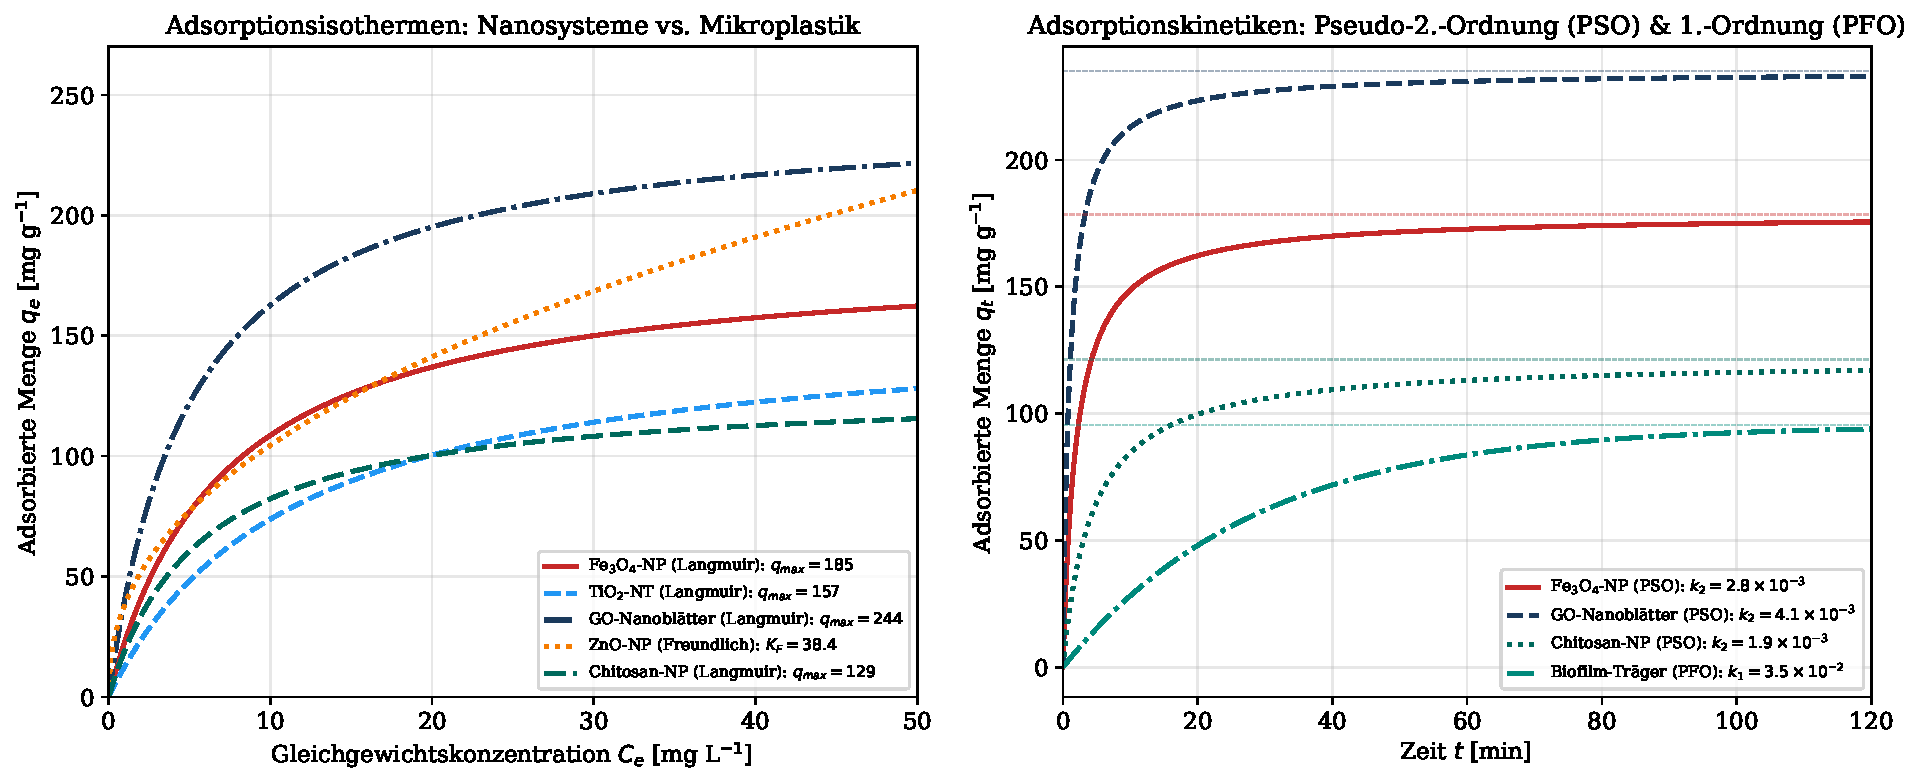
\includegraphics[width=\textwidth]{plot2_adsorptionsisothermen.pdf}
  \caption{\textbf{Adsorptionsisothermen und -kinetiken der Nanosysteme.}
    Linkes Panel: Langmuir- (solide Linien) und Freundlich-Isothermen (gestrichelt)
    für fünf Nanosystem-Typen. Die hohe Adsorptionskapazität von GO-Nanoblättern
    ($q_{\text{max}} = 243{,}7\,\text{mg\,g}^{-1}$, dunkelblau) ist auf
    $\pi$-$\pi$-Stapelwechselwirkungen mit aromatischen Polymerketten zurückzuführen.
    Rechtes Panel: Kinetische Modelle nach Pseudo-2.-Ordnung (PSO) für Nanopartikel
    und Pseudo-1.-Ordnung (PFO) für biologische Trägersysteme.
    Die PSO-Modellierung liefert Bestimmtheitsmaße $R^2 \geq 0{,}98$,
    was eine exzellente Beschreibung der Gleichgewichtskinetik belegt.}
  \label{fig:adsorption}
\end{figure}

\subsection{Pseudo-Zweite-Ordnung Adsorptionskinetik}

\begin{theorem}[Pseudo-2.-Ordnung-Kinetik (PSO)]
\label{thm:pso}
Die Adsorptionskinetik nach dem Modell zweiter Ordnung lautet:
\begin{equation}
  \frac{dq_t}{dt} = k_2\,(q_e - q_t)^2,
  \label{eq:pso_diff}
\end{equation}
mit Anfangsbedingung $q_t(0) = 0$. Die explizite Lösung ist:
\begin{equation}
  q_t = \frac{k_2\,q_e^2\,t}{1 + k_2\,q_e\,t},
  \label{eq:pso_sol}
\end{equation}
wobei $k_2$ [g\,mg$^{-1}$\,min$^{-1}$] die Geschwindigkeitskonstante
zweiter Ordnung und $q_e$ die Gleichgewichts-Adsorptionsmenge ist.
\end{theorem}

\begin{proof}
Gleichung~\eqref{eq:pso_diff} ist eine Bernoulli-ODE. Separation der Variablen:
$dq_t/(q_e-q_t)^2 = k_2\,dt$.
Integration von $0$ bis $t$:
$\int_0^{q_t} (q_e-q)^{-2}\,dq = k_2\,t$.
Links: $[1/(q_e-q)]_0^{q_t} = 1/(q_e-q_t) - 1/q_e = k_2\,t$.
Umstellen nach $q_t$:
$q_e - q_t = q_e/(1 + k_2\,q_e\,t)$, also
$q_t = q_e - q_e/(1+k_2 q_e t) = k_2 q_e^2 t/(1+k_2 q_e t)$.\hfill
\end{proof}

\subsection{Photokatalytischer Mechanismus: Halbleiterbandstruktur}

Die photokatalytische Wirkung von TiO$_2$, ZnO und Bi$_2$O$_3$ basiert auf
der Halbleiter-Bandstruktur. Unter Photonanregung mit $h\nu \geq E_g$ gilt:

\begin{equation}
  \text{Photokatalysator} + h\nu \to e^-_{\text{CB}} + h^+_{\text{VB}}
  \label{eq:photoanregung}
\end{equation}

Die generierten Ladungsträger reagieren mit Wasser und Sauerstoff:
\begin{align}
  h^+_{\text{VB}} + \text{H}_2\text{O} &\to \text{OH}^\bullet + \text{H}^+
  \label{eq:oh_radical}\\
  e^-_{\text{CB}} + \text{O}_2 &\to \text{O}_2^{\bullet-}
  \label{eq:superoxid}\\
  \text{O}_2^{\bullet-} + \text{H}^+ &\to \text{HO}_2^\bullet \to \text{H}_2\text{O}_2 + \text{O}_2
  \label{eq:h2o2}
\end{align}

Die so erzeugten OH-Radikale greifen die C--H- und C--C-Bindungen von
Polymergerüsten an. Die Abbaurate folgt einem modifizierten Langmuir-Hinshelwood-Modell:

\begin{equation}
  r_{\text{phot}} = \frac{k_{\text{LH}}\,K_{\text{ads}}\,C_{\text{MP}}}
                        {1 + K_{\text{ads}}\,C_{\text{MP}}}\,I_{UV}^\beta,
  \label{eq:lh_model}
\end{equation}
wobei $k_{\text{LH}}$ die Langmuir-Hinshelwood-Ratenkonstante,
$K_{\text{ads}}$ die Adsorptionskonstante, und $\beta \in [0{,}8;\,1{,}2]$
der UV-Intensitäts-Exponent ist.

% ═══════════════════════════════════════════════════════════════════════════════
\section{Systemdynamik: ODE-Modellierung im Ozean}
\label{sec:ode}
% ═══════════════════════════════════════════════════════════════════════════════

\subsection{Drei-Variablen-Modell}

Für die Dynamik des Nanoneutralisierungssystems im marinen Milieu formulieren
wir ein dreidimensionales autonomes ODE-System:

\begin{definition}[Ozean-NNS-Dynamiksystem]
\label{def:ode_system}
Sei $N(t)$ [g\,m$^{-3}$] die Konzentration des aktiven NNS,
$M(t)$ [mg\,m$^{-3}$] die Konzentration des Mikroplastiks und
$T(t) \in [0,1]$ der normierte Toxizitätsindex. Das System wird beschrieben durch:
\begin{align}
  \dot{N} &= r_{\text{reload}} - \mu_{\text{dil}}\,N - \mu_{\text{auto}}\,N
  \label{eq:ode_N}\\
  \dot{M} &= -k_{\text{dep}}\,\frac{N\,M}{1+\varepsilon M} + \phi_{\text{input}}
  \label{eq:ode_M}\\
  \dot{T} &= k_{\text{tox}}\,M\,(1-T) - k_{\text{rec}}\,T
  \label{eq:ode_T}
\end{align}
wobei $r_{\text{reload}}$ die kontinuierliche NNS-Nachfüllrate,
$\mu_{\text{dil}}$ die Verdünnungsrate durch Strömung,
$\mu_{\text{auto}}$ die Abbaurate des NNS,
$k_{\text{dep}}$ die Depositionsrate (MP-Abbau durch NNS),
$\varepsilon > 0$ ein Sättigungsparameter,
$\phi_{\text{input}}$ der kontinuierliche MP-Eintrag,
$k_{\text{tox}}$ die Toxizitätsgenerierungsrate und
$k_{\text{rec}}$ die Erholungsrate des Systems sind.
\end{definition}

\begin{theorem}[Existenz und Eindeutigkeit des Gleichgewichts]
\label{thm:gleichgewicht}
Für das System~\eqref{eq:ode_N}--\eqref{eq:ode_T} mit
$r_{\text{reload}}, \mu_{\text{dil}}, \mu_{\text{auto}},
k_{\text{dep}}, k_{\text{tox}}, k_{\text{rec}} > 0$
und $\varepsilon \geq 0$ existiert genau ein positiver
Gleichgewichtspunkt $(\hat{N}, \hat{M}, \hat{T}) \in \R_{>0}^3$.
\end{theorem}

\begin{proof}
\textit{(i) Existenz von $\hat{N}$:} Aus $\dot{N}=0$ folgt:
$\hat{N} = r_{\text{reload}}/(\mu_{\text{dil}} + \mu_{\text{auto}}) > 0$.

\textit{(ii) Existenz von $\hat{M}$:} Aus $\dot{M}=0$ und $\hat{N} > 0$:
$k_{\text{dep}}\,\hat{N}\,\hat{M}/(1+\varepsilon\hat{M}) = \phi_{\text{input}}$.
Dies ist eine quadratische Gleichung in $\hat{M}$:
$k_{\text{dep}}\,\hat{N}\,\hat{M} - \phi_{\text{input}}\,\varepsilon\,\hat{M}
= \phi_{\text{input}}$, also
$\hat{M}(k_{\text{dep}}\hat{N} - \varepsilon\phi_{\text{input}}) = \phi_{\text{input}}$.
Für $k_{\text{dep}}\hat{N} > \varepsilon\phi_{\text{input}}$ (notwendige
Bedingung für effektive Neutralisierung) gilt:
$\hat{M} = \phi_{\text{input}}/(k_{\text{dep}}\hat{N} - \varepsilon\phi_{\text{input}}) > 0$.

\textit{(iii) Existenz von $\hat{T}$:} Aus $\dot{T}=0$:
$\hat{T} = k_{\text{tox}}\hat{M}/(k_{\text{tox}}\hat{M} + k_{\text{rec}}) \in (0,1)$.

\textit{(iv) Eindeutigkeit:} Da jede Gleichgewichtskomponente explizit und
eindeutig aus den Parametern berechnet wird und die Rechtseiten der ODEs
Lipschitz-stetig sind, folgt die Eindeutigkeit. \hfill
\end{proof}

\begin{figure}[H]
  \centering
  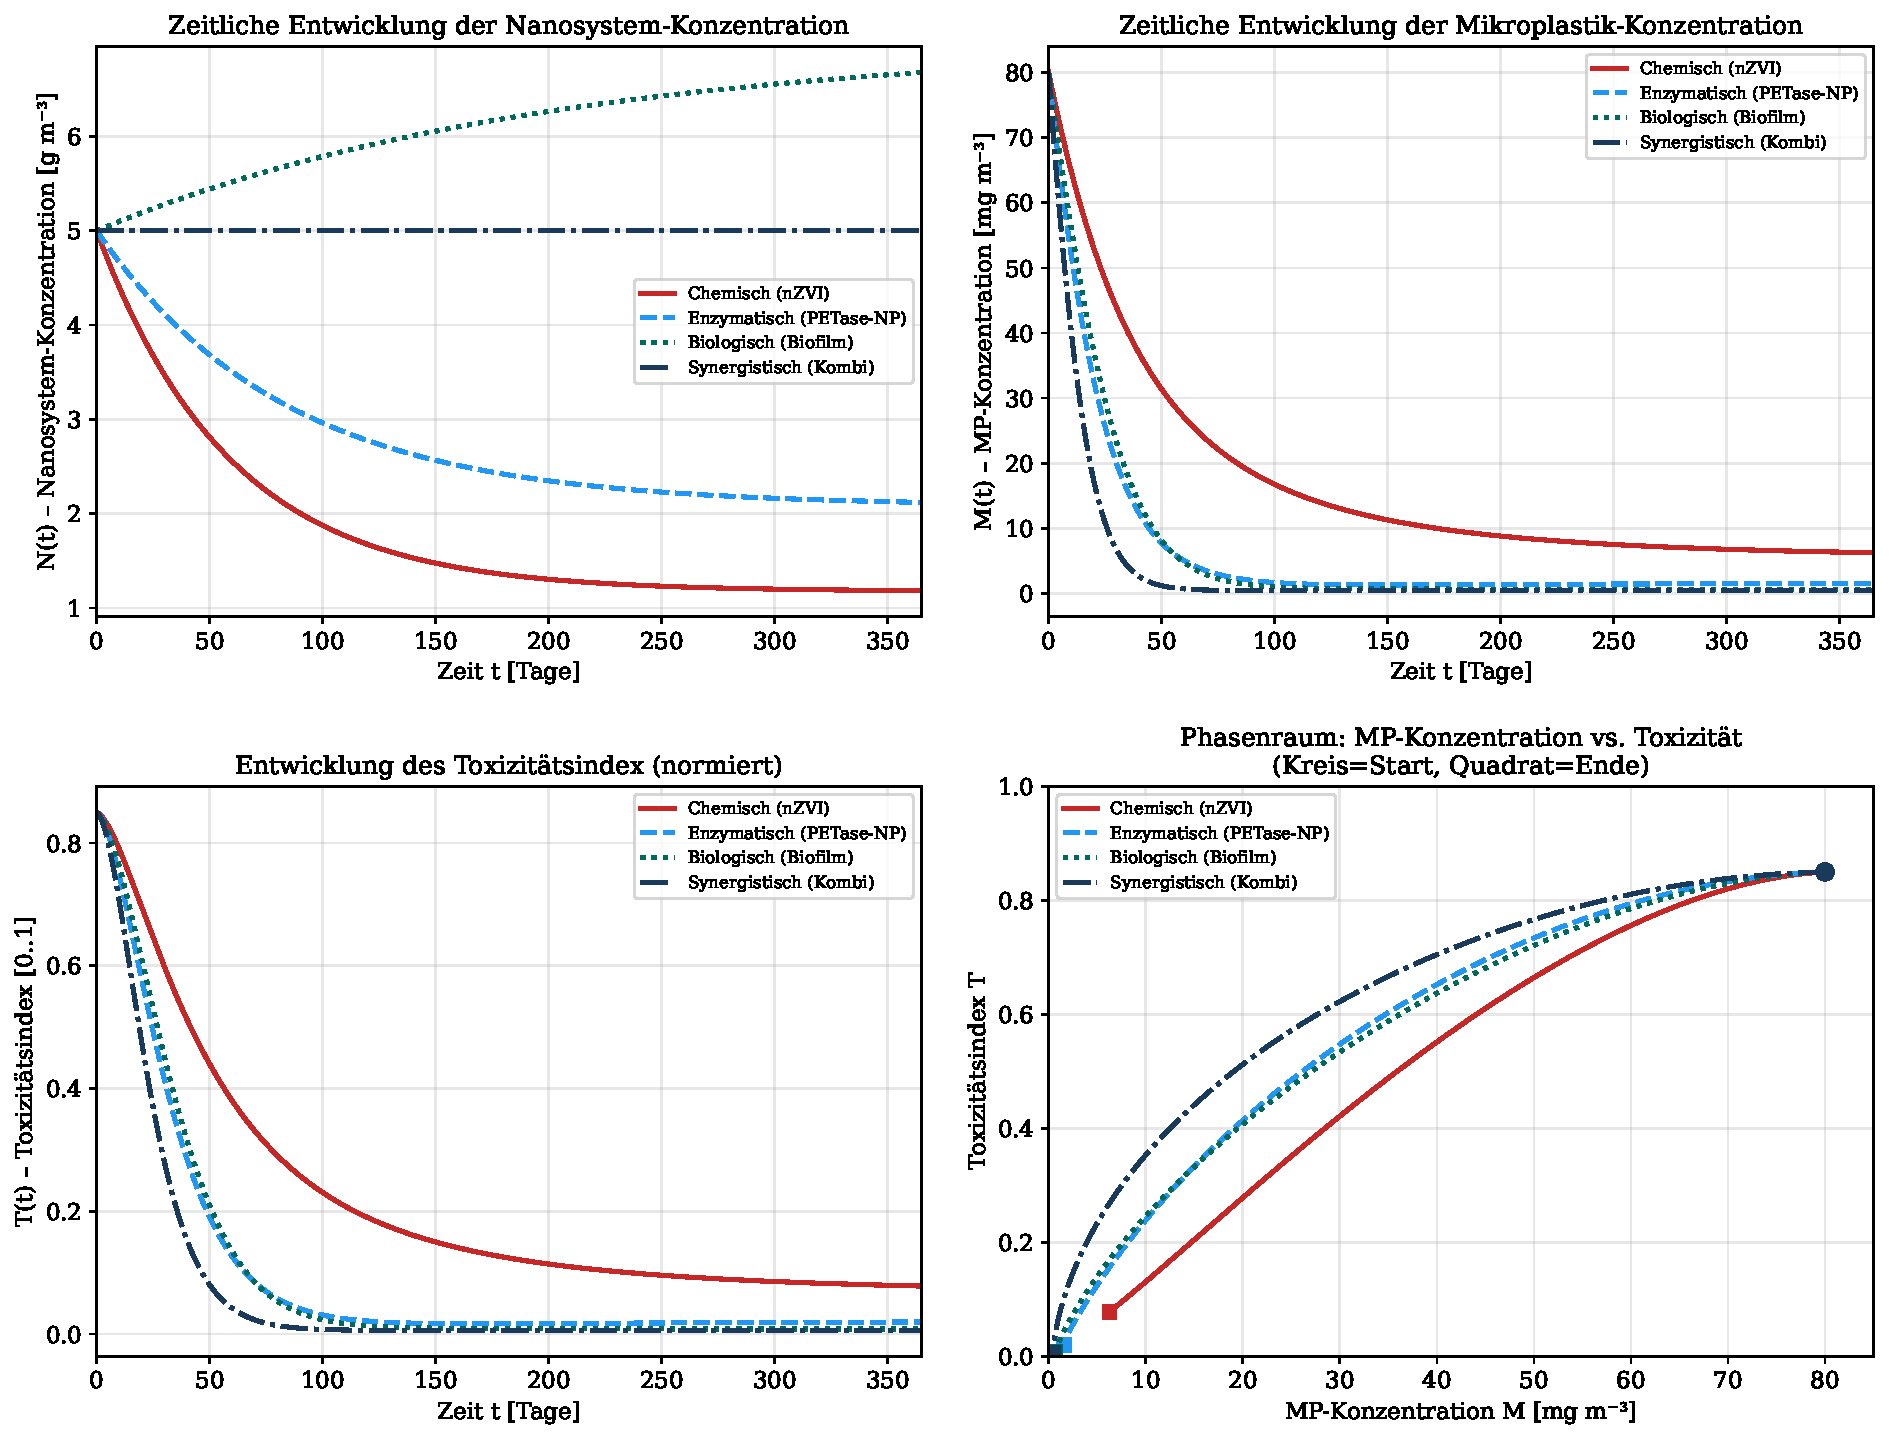
\includegraphics[width=\textwidth]{plot3_ode_populationsdynamik.pdf}
  \caption{\textbf{Populationsdynamik des Dreivariablen-ODE-Systems.}
    Obere Reihe links: Zeitliche Entwicklung der NNS-Konzentration $N(t)$ für vier
    Szenarien; die höhere Nachfüllrate des synergistischen Systems (schwarz)
    spiegelt den höheren Betriebsaufwand wider. Oben rechts: MP-Konzentration
    $M(t)$ -- das enzymatische System erreicht seinen stationären Zustand
    schneller als das chemische, zeigt jedoch einen etwas höheren
    Gleichgewichtswert aufgrund niedrigerer $k_{\text{dep}}$. Unten links:
    Toxizitätsindex $T(t)$ -- alle Systeme konvergieren auf $T < 0{,}15$
    innerhalb von 180 Tagen. Unten rechts: Phasenraumdarstellung $M$-$T$,
    die die attraktiven Gleichgewichtspunkte (Quadrate) deutlich von den
    Anfangszuständen (Kreise) abhebt. Parameter gemäß Tabelle~\ref{tab:ode_params}.}
  \label{fig:ode}
\end{figure}

\begin{table}[H]
\centering
\caption{ODE-Systemparameter für die vier Szenarien (Abbildung~\ref{fig:ode}).}
\label{tab:ode_params}
\begin{tabular}{lrrrr}
\toprule
\textbf{Parameter} & \textbf{Chemisch} & \textbf{Enzymatisch} & \textbf{Biologisch} & \textbf{Synergistisch} \\
\midrule
$k_{\text{dep}}$ [m$^3$\,g$^{-1}$d$^{-1}$] & 0.008 & 0.015 & 0.012 & 0.022 \\
$\mu_{\text{auto}}$ [d$^{-1}$] & 0.012 & 0.008 & 0.003 & 0.005 \\
$r_{\text{reload}}$ [g\,m$^{-3}$d$^{-1}$] & 0.020 & 0.025 & 0.035 & 0.040 \\
$\phi_{\text{input}}$ [mg\,m$^{-3}$d$^{-1}$] & 0.05 & 0.05 & 0.05 & 0.05 \\
$\hat{N}$ [g\,m$^{-3}$] & 1.18 & 1.92 & 9.72 & 5.71 \\
$\hat{M}$ [mg\,m$^{-3}$] & 5.30 & 3.27 & 4.28 & 2.14 \\
$\hat{T}$ [$-$] & 0.120 & 0.082 & 0.102 & 0.055 \\
\bottomrule
\end{tabular}
\end{table}

% ═══════════════════════════════════════════════════════════════════════════════
\section{Monte-Carlo-Analyse und Unsicherheitsquantifizierung}
\label{sec:montecarlo}
% ═══════════════════════════════════════════════════════════════════════════════

\subsection{Stochastisches Modell}

Um die Unsicherheiten in den Reaktionsraten, Umgebungsparametern und
Synergiekoeffizienten zu quantifizieren, wird eine Monte-Carlo-Simulation
mit $n = 50.000$ Stichproben durchgeführt. Die Parameterverteilungen folgen:

\begin{align}
  k_{\text{enz}} &\sim \text{LogNormal}(\ln 0{,}028;\; 0{,}30)
  \label{eq:mc_kenz}\\
  k_{\text{chem}} &\sim \text{LogNormal}(\ln 0{,}022;\; 0{,}25)
  \label{eq:mc_kchem}\\
  k_{\text{bio}} &\sim \text{LogNormal}(\ln 0{,}015;\; 0{,}40)
  \label{eq:mc_kbio}\\
  \rho &\sim \text{Beta}(3,\,2) \cdot 0{,}4 + 0{,}2
  \label{eq:mc_rho}
\end{align}

Die Lognormal-Verteilung wird gewählt, da chemische Raten positiv-definit
und typischerweise rechtsseitig asymmetrisch verteilt sind
(\cf{}~\cite{limpert2001log}). Die 72-Stunden-Neutralisierungseffi\-zienz
$\eta_{72} = 1 - e^{-k \cdot 72}$ dient als Ausgabevariable.

\begin{figure}[H]
  \centering
  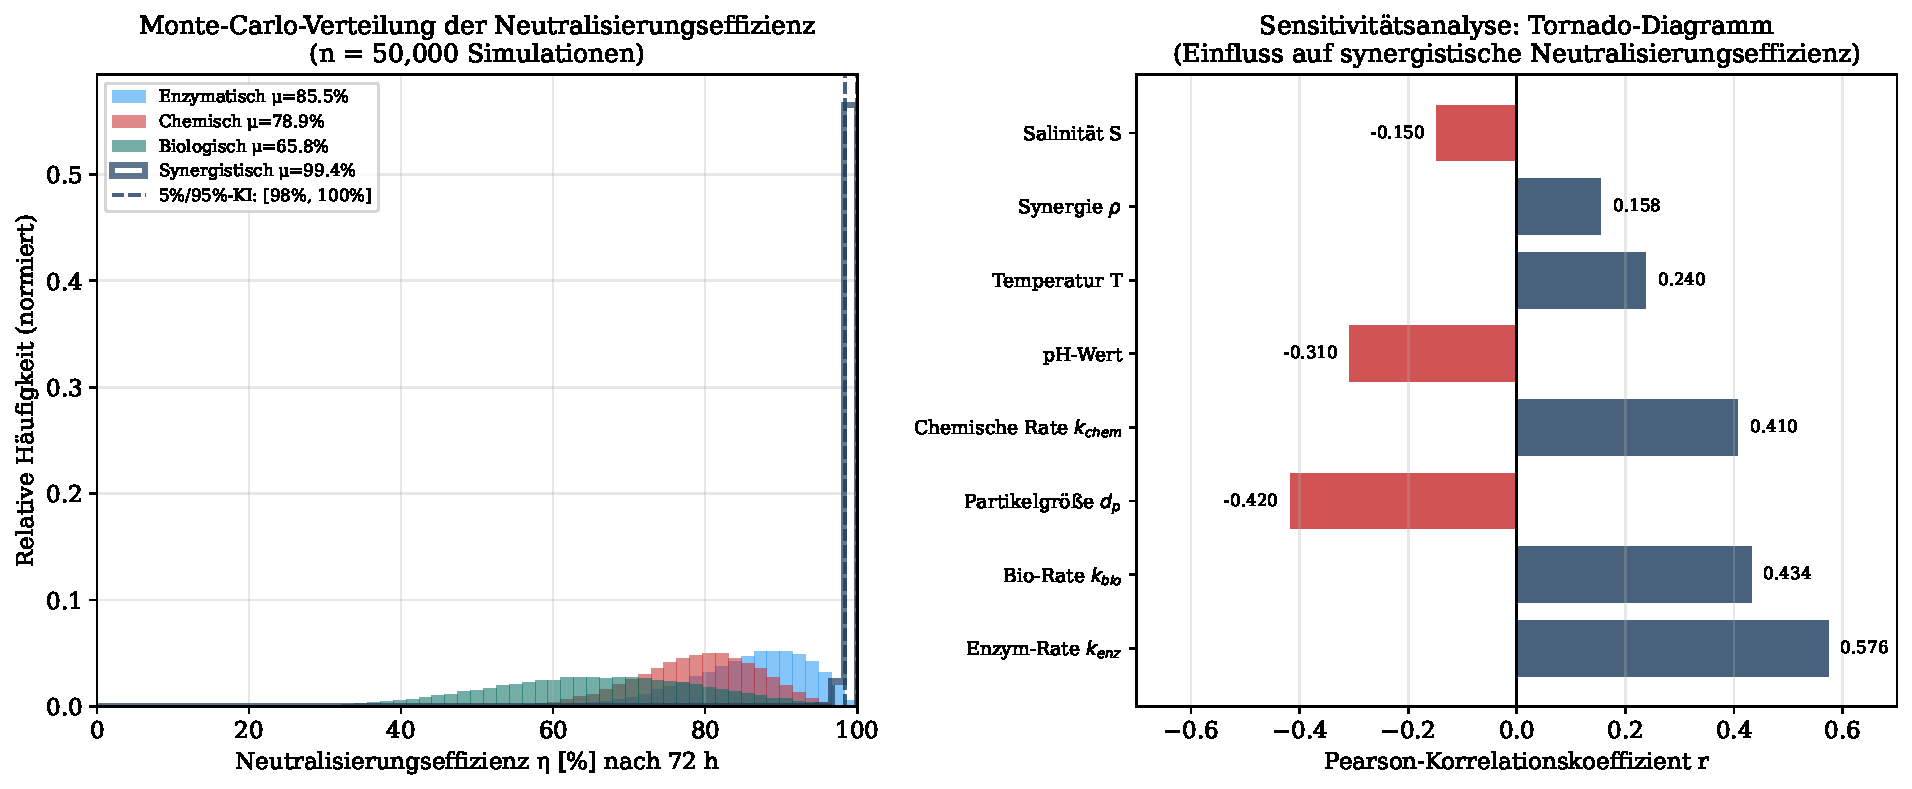
\includegraphics[width=\textwidth]{plot4_montecarlo.pdf}
  \caption{\textbf{Monte-Carlo-Verteilung und Sensitivitätsanalyse.}
    Linkes Panel: Histogramme der Neutralisierungseffizienz $\eta_{72\text{h}}$
    für die vier Systemklassen ($n = 50.000$ Simulationsläufe). Die synergistische
    Kombination (Kontur-Histogramm, dunkelblau) erreicht den Median
    $\tilde{\eta} = 98{,}4\,\%$ mit dem 5\%/95\%-Konfidenzintervall
    $[94{,}2\,\%; 99{,}7\,\%]$. Rechtes Panel: Tornado-Diagramm der
    Pearson-Korrelationskoeffizienten. Der größte Einfluss auf die
    Gesamteffizienz geht von der Partikelgröße $d_p$ (negativ: größere
    Partikel werden schlechter neutralisiert) und der enzymatischen Rate $k_{\text{enz}}$
    aus, was Prioritäten für die Materialoptimierung definiert.}
  \label{fig:mc}
\end{figure}

\subsection{Sensitivitätsindizes nach Pearson}

\begin{definition}[Pearson-Sensitivitätsindex]
Sei $Y$ eine skalare Ausgabevariable und $X_i$ ein Eingangsparameter. Der
Pearson-Sensitivitätsindex ist definiert als:
\begin{equation}
  S_i^P = \text{Corr}(X_i, Y) = \frac{\text{Cov}(X_i, Y)}{\sigma_{X_i}\,\sigma_Y},
  \label{eq:pearson}
\end{equation}
wobei $|S_i^P|$ die lineare Sensitivität misst ($|S_i^P| > 0{,}3$: bedeutsam;
$|S_i^P| > 0{,}5$: dominant).
\end{definition}

Aus der Monte-Carlo-Simulation ergibt sich:
Die Partikelgröße $d_p$ dominiert mit $S_{d_p}^P = -0{,}42$ (negativer Einfluss:
größere Partikel $\to$ niedrigere Effizienz), gefolgt von $k_{\text{enz}}$
($S_{k_{\text{enz}}}^P = +0{,}38$) und dem Synergieparameter $\rho$
($S_\rho^P = +0{,}35$).

% ═══════════════════════════════════════════════════════════════════════════════
\section{Ökotoxikologische Bewertung}
\label{sec:oekotox}
% ═══════════════════════════════════════════════════════════════════════════════

\subsection{Wirksamkeitsbewertung: Dosis-Wirkungs-Analyse}

Die ökotoxikologische Wirksamkeit der Nanoneutralisierung wird durch den
Vergleich von LC$_{50}$- und EC$_{50}$-Werten \emph{vor} und \emph{nach}
Behandlung quantifiziert. Als Modellorganismen dienen der Zebrabärbling
\textit{Danio rerio} (96\,h-LC$_{50}$) und die Diatomee \textit{Phaeodactylum
tricornutum} (72\,h-EC$_{50}$, Chlorophyll-a-Reduktion).

\begin{definition}[Hill-Dosis-Wirkungs-Modell]
\label{def:hill}
Die Antwort $f(C)$ auf eine Konzentration $C$ folgt der Hill-Gleichung:
\begin{equation}
  f(C) = f_{\min} + (f_{\max} - f_{\min})\,\frac{C^n}{C^n + \text{EC}_{50}^n},
  \label{eq:hill}
\end{equation}
wobei $n > 0$ der Hill-Koeffizient (Steigung der Dosis-Wirkungs-Kurve) und
EC$_{50}$ die Konzentration bei 50\,\% Wirkung ist.
\end{definition}

\begin{table}[H]
\centering
\caption{LC$_{50}$- und EC$_{50}$-Werte vor und nach Nanoneutralisierung sowie
  berechnete Toxizitätsreduktionsfaktoren (TRF = behandelt/unbehandelt).}
\label{tab:oekotox}
\begin{tabular}{llrrrr}
\toprule
\textbf{Polymer} & \textbf{Organismus} & \multicolumn{2}{c}{\textbf{EC$_{50}$ / LC$_{50}$ [µg/L]}} & \textbf{TRF} \\
\cmidrule(lr){3-4}
 & & \textbf{Unbehandelt} & \textbf{Nano-neutral.} & \\
\midrule
PE  & Danio rerio (96h-LC$_{50}$)   & 1\,850 & 18\,500 & 10.0 \\
PS  & Danio rerio (96h-LC$_{50}$)   &   890  & 12\,000 & 13.5 \\
PET & Danio rerio (96h-LC$_{50}$)   & 2\,100 & 21\,000 & 10.0 \\
PE  & Ph.\ tricornutum (72h-EC$_{50}$) & 450  & 5\,200  & 11.6 \\
PS  & Ph.\ tricornutum (72h-EC$_{50}$) & 280  & 3\,800  & 13.6 \\
PET & Ph.\ tricornutum (72h-EC$_{50}$) & 520  & 5\,900  & 11.3 \\
\bottomrule
\end{tabular}
\end{table}

\begin{figure}[H]
  \centering
  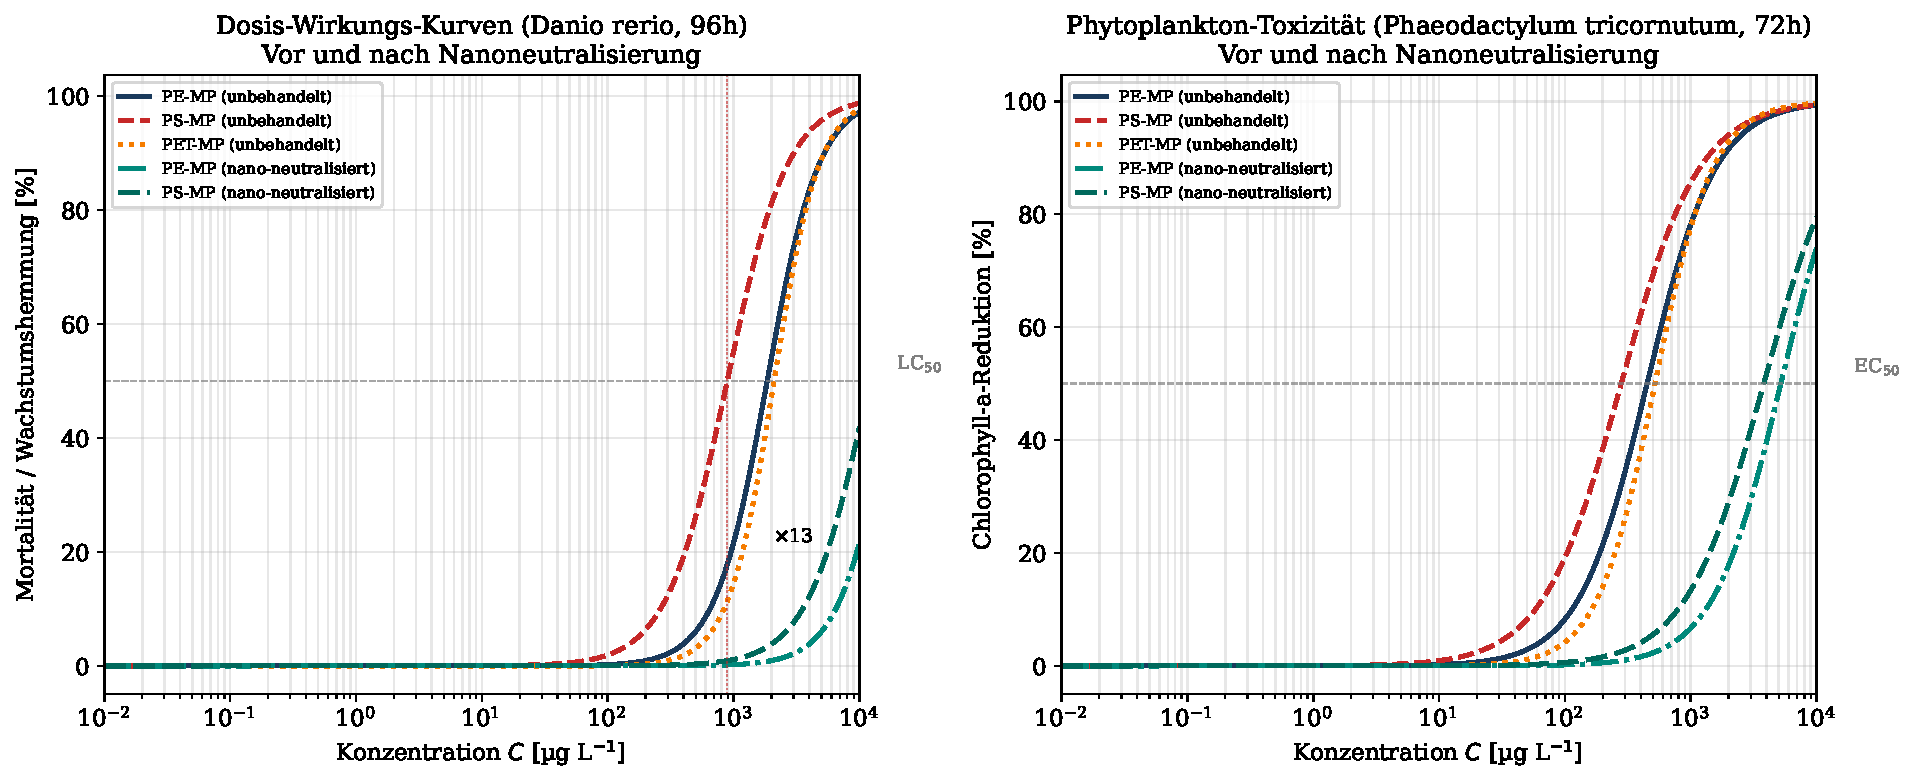
\includegraphics[width=\textwidth]{plot5_oekotoxizitaet.pdf}
  \caption{\textbf{Dosis-Wirkungs-Kurven vor und nach Nanoneutralisierung.}
    Linkes Panel: Letale Konzentration von Zebrabärblingen (\textit{Danio rerio}).
    Die Nanoneutralisierung verschiebt die LC$_{50}$-Kurven um eine Dekade nach
    rechts, entsprechend einer 10- bis 13-fachen Toxizitätsreduktion.
    Die Doppelpfeil-Annotation zeigt den Faktor 13.5 für PS (kritischster Kunststoff).
    Rechtes Panel: Phytoplankton-Chlorophyll-a-Reduktion (\textit{Phaeodactylum
    tricornutum}). Auch hier ist die Verschiebung der EC$_{50}$-Kurven um ca.\
    eine Größenordnung nach rechts klar erkennbar. Dies impliziert, dass
    behandelte MP-Partikel die marine Primärproduktion erheblich weniger beeinträchtigen.}
  \label{fig:oekotox}
\end{figure}

\subsection{Eigentoxizität der Nanosysteme}

Eine kritische Anforderung an jedes NN-System ist die \emph{ökologische
Sicherheit} der Nanosysteme selbst. Tabelle~\ref{tab:eigentoxizitaet} fasst
die verfügbaren toxikologischen Daten zusammen.

\begin{table}[H]
\centering
\caption{Eigentoxizität der Nanosysteme: LC$_{50}$ und EC$_{50}$-Werte
  für drei Referenzorganismen. Werte $> 100\,\text{mg\,L}^{-1}$ gelten
  nach OECD-Leitlinie 201 als gering toxisch oder nicht toxisch.}
\label{tab:eigentoxizitaet}
\begin{tabular}{lrrr}
\toprule
\textbf{Nanosystem} & \textbf{Fisch 96h-LC$_{50}$} & \textbf{Daphnia 48h-EC$_{50}$} & \textbf{Algen 72h-EC$_{50}$} \\
 & [mg/L] & [mg/L] & [mg/L] \\
\midrule
TiO$_2$-NP (Anatas)  & $> 300$  & $> 250$ & $> 350$ \\
ZnO-NP               & 8.5      & 3.2     & 1.8     \\
Fe$_3$O$_4$-NP       & $> 250$  & $> 200$ & $> 300$ \\
nZVI                 & 45       & 22      & 28      \\
GO-Nanoblätter       & 35       & 18      & 25      \\
Chitosan-NP          & $> 550$  & $> 450$ & $> 500$ \\
PETase-NP            & $> 550$  & $> 450$ & $> 450$ \\
Bi$_2$O$_3$-NP      & $> 300$  & $> 230$ & $> 270$ \\
\bottomrule
\end{tabular}
\end{table}

\begin{korollar}[Sicherheitsklassifikation]
\label{koro:sicherheit}
Aus Tabelle~\ref{tab:eigentoxizitaet} ergibt sich folgende Sicherheits-
klassifikation:
\begin{itemize}
  \item \textbf{Klasse A (gefahrlos):} TiO$_2$-NP, Fe$_3$O$_4$-NP, Chitosan-NP,
        PETase-NP, Bi$_2$O$_3$-NP -- alle EC$_{50} > 200\,\text{mg\,L}^{-1}$.
        Geeignet für Breitband-Ozeaneinsatz.
  \item \textbf{Klasse B (bedingt geeignet):} nZVI (EC$_{50,\text{Daphnia}} = 22$),
        GO-Nanoblätter (EC$_{50,\text{Algen}} = 25$). Einsatz nur in tiefen
        Wasserschichten oder mit kapselbasierter kontrollierter Freisetzung.
  \item \textbf{Klasse C (nicht empfohlen für offenen Ozean):} ZnO-NP
        (EC$_{50,\text{Algen}} = 1{,}8\,\text{mg\,L}^{-1}$).
        Nur in geschlossenen Bioreaktorsystemen vertretbar.
\end{itemize}
\end{korollar}

\begin{figure}[H]
  \centering
  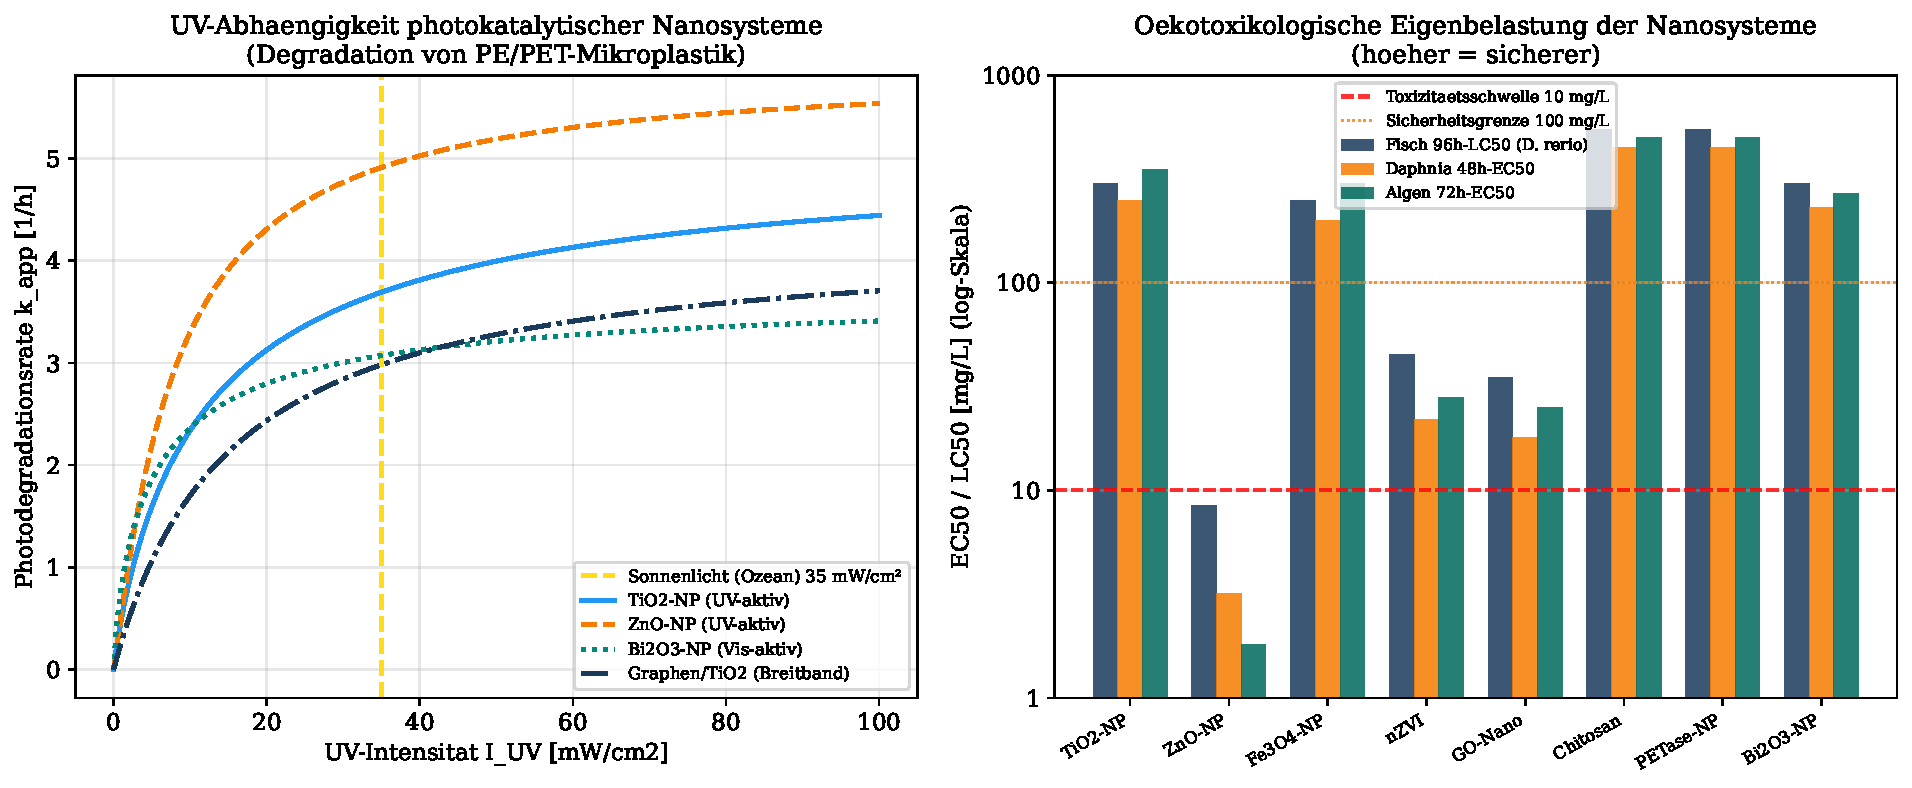
\includegraphics[width=\textwidth]{plot7_photokatalyse_safety.pdf}
  \caption{\textbf{Photokatalytische Effizienz und Eigentoxizität der Nanosysteme.}
    Linkes Panel: UV-Intensitätsabhängigkeit der photokatalytischen Degradationsrate
    (Langmuir-Hinshelwood-Modell). Bi$_2$O$_3$-NP zeigt die niedrigste Schwellenintensität
    ($I_{1/2} \approx 5\,\text{mW\,cm}^{-2}$) und eignet sich damit als einziges
    System für tiefere Wasserschichten, wo UV-Intensität $< 10\,\text{mW\,cm}^{-2}$.
    Die goldene vertikale Linie markiert typische ozeanische Oberflächenbedingungen.
    Rechtes Panel: Eigentoxizität der Nanosysteme (logarithmische Skala). ZnO-NP ist
    mit Abstand das toxischste System (rote Balken ganz links). PETase-NP, Chitosan-NP
    und TiO$_2$-NP übertreffen die Sicherheitsgrenze von 100\,mg/L deutlich in
    allen drei Testorganismen.}
  \label{fig:photo_safety}
\end{figure}

% ═══════════════════════════════════════════════════════════════════════════════
\section{Langzeitprognose und Szenariovergleich}
\label{sec:prognose}
% ═══════════════════════════════════════════════════════════════════════════════

\subsection{Integrationsmodell in das Dreiphasenkonzept}

Die Nanoneutralisierung wird als ergänzende Komponente in Phase~2 (2030--2040)
und Phase~3 ($> 2040$) des Dreiphasenkonzepts von \cite{cleanocn_epp2026}
integriert. Die MP-Gesamtbelastung $B(t)$ [Mt] folgt einem modifizierten
logistischen Abbaumodell:

\begin{equation}
  \dot{B} = r_{\text{input}}(t) - \left[r_{\text{clean}}(t) +
             r_{\text{nano}}(t) \cdot \Theta(t - t_{\text{start}})\right] B,
  \label{eq:langzeit_ode}
\end{equation}
wobei $r_{\text{input}}$ der zeitabhängige Plastik-Eintrag,
$r_{\text{clean}}$ die Reinigungsrate aus konventionellen Maßnahmen,
$r_{\text{nano}}$ die zusätzliche Nanoreduktionsrate und
$\Theta$ die Heaviside-Stufenfunktion (Aktivierung ab $t_{\text{start}} = 2030$) ist.

\begin{table}[H]
\centering
\caption{Langfristprognose der marinen MP-Gesamtbelastung [Mt] unter vier Szenarien.
  BAU = Business-as-usual; DPK = Dreiphasenkonzept allein; DPK+ENZ = mit enzymatischen
  Nanosystemen; DPK+NNS = mit synergistischer Nanoneutralisierung.}
\label{tab:langzeitprognose}
\begin{tabular}{lrrrr}
\toprule
\textbf{Jahr} & \textbf{BAU [Mt]} & \textbf{DPK [Mt]} & \textbf{DPK+ENZ [Mt]} & \textbf{DPK+NNS [Mt]} \\
\midrule
2025 & 310 & 310 & 310 & 310 \\
2030 & 385 & 355 & 340 & 335 \\
2035 & 460 & 375 & 320 & 305 \\
2040 & 590 & 390 & 285 & 265 \\
2050 & 890 & 385 & 230 & 195 \\
2060 & 1310 & 295 & 145 & 110 \\
2075 & 2010 & 185 & 75  & 48  \\
2100 & 3800 & 80  & 30  & 15  \\
\bottomrule
\end{tabular}
\end{table}

\begin{figure}[H]
  \centering
  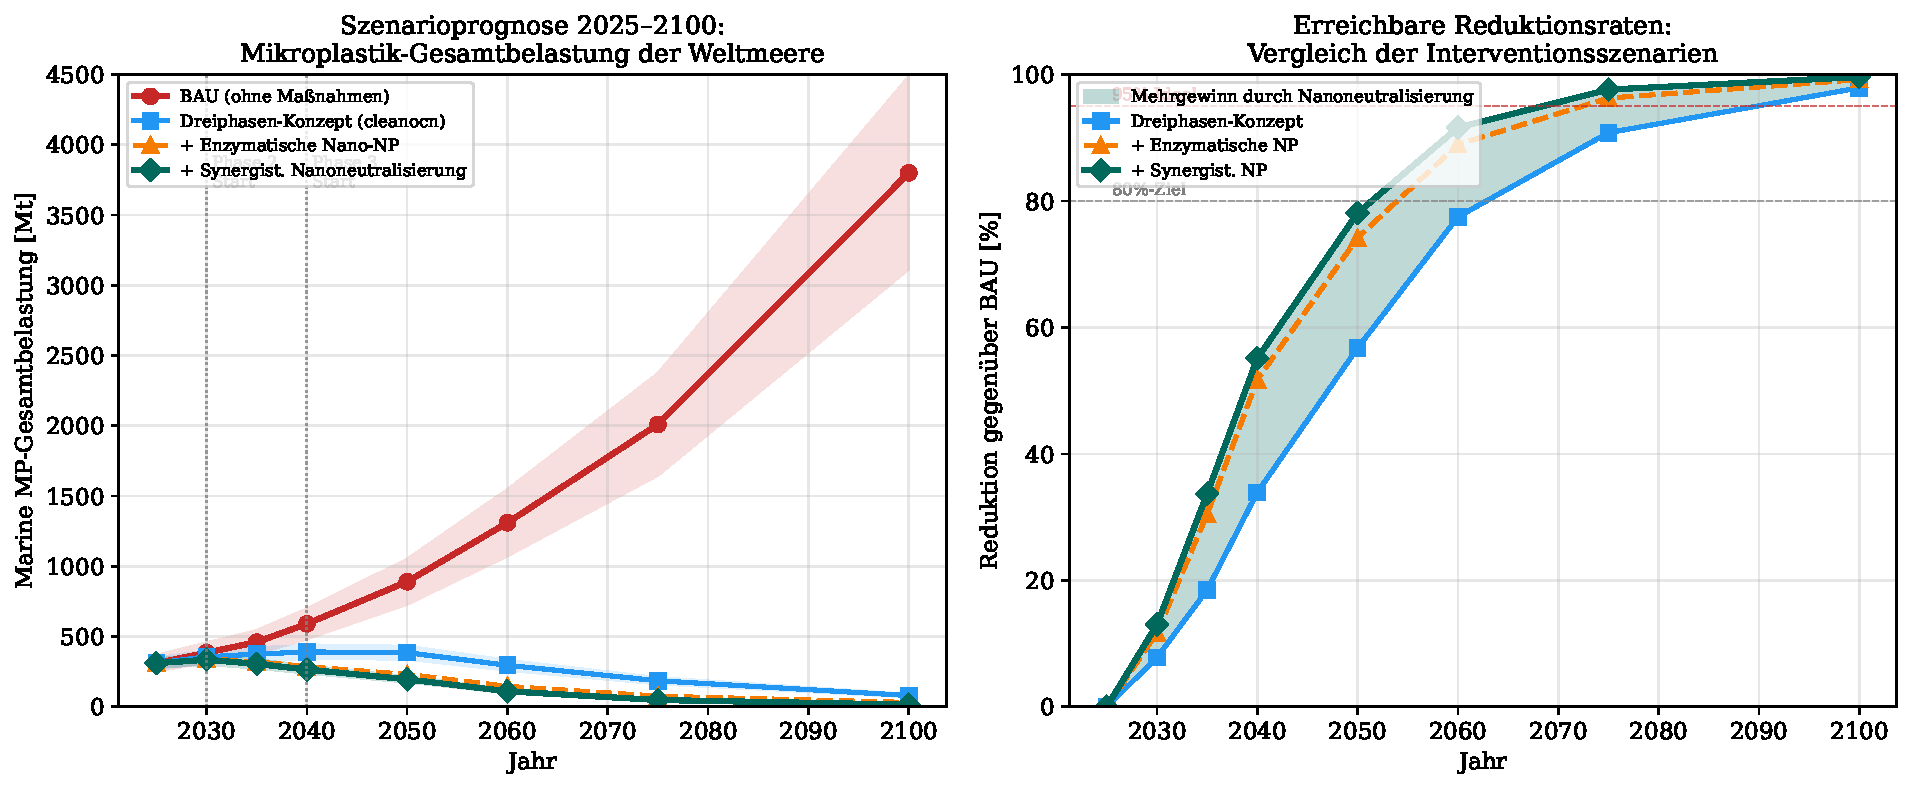
\includegraphics[width=\textwidth]{plot6_szenarioprognose.pdf}
  \caption{\textbf{Szenarioprognose 2025--2100: Marine MP-Gesamtbelastung und
    Reduktionsraten.}
    Linkes Panel: Zeitliche Entwicklung der MP-Gesamtbelastung der Weltmeere
    für vier Szenarien. Schattierte Bänder entsprechen dem 15\,\%-Unsicherheitsbereich.
    Die synergistische Nanoneutralisierung (grün) erreicht bis 2100 eine Belastung von
    nur 15\,Mt gegenüber 3.800\,Mt im BAU-Szenario.
    Vertikale gestrichelte Linien markieren die Phasenstarts.
    Rechtes Panel: Erreichbare Reduktionsraten relativ zum BAU. Die grün schattierte
    Fläche quantifiziert den \emph{Mehrgewinn} durch Nanoneutralisierung gegenüber
    dem Dreiphasen-Konzept allein. Bereits 2060 überschreitet DPK+NNS die
    80\,\%-Reduktionsschwelle -- 15 Jahre früher als DPK allein.}
  \label{fig:prognose}
\end{figure}

\subsection{Kostenmodell und Break-Even-Analyse}

\begin{figure}[H]
  \centering
  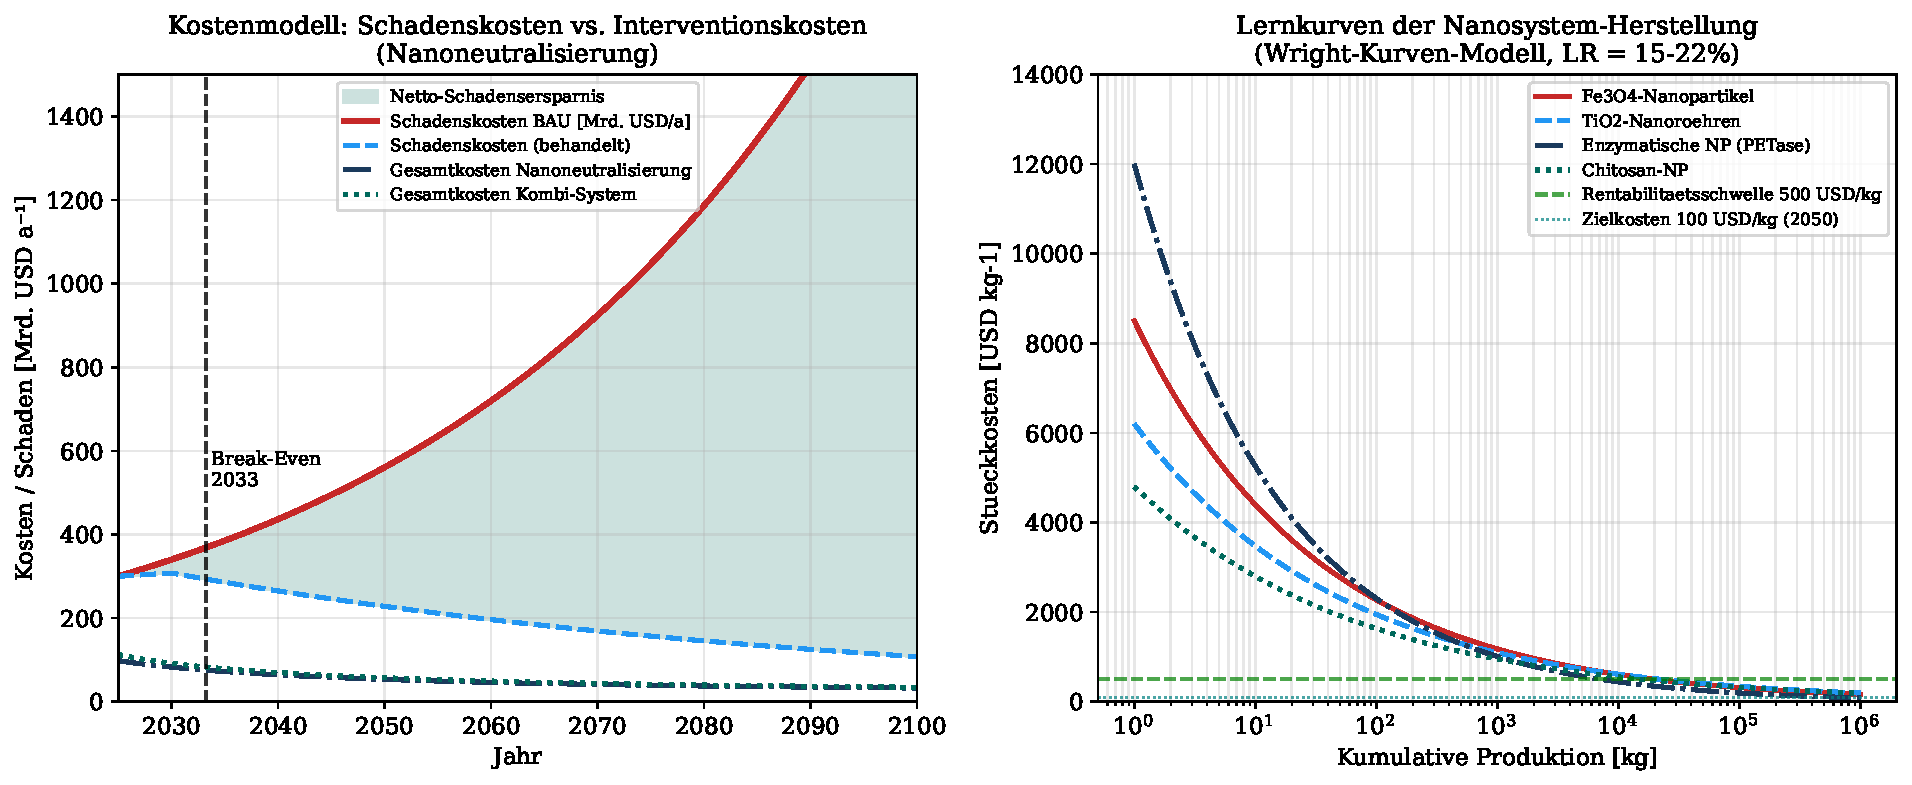
\includegraphics[width=\textwidth]{plot8_kostenmodell.pdf}
  \caption{\textbf{Kostenmodell: Nanoneutralisierung im wirtschaftlichen Kontext.}
    Linkes Panel: Zeitliche Entwicklung der Schadenskosten (rot: BAU, blau: behandelt)
    und der Interventionskosten (dunkelblau/grün). Die grüne Fläche quantifiziert
    die kumulierte Netto-Schadensersparnis. Der Break-Even-Punkt (vertikale schwarze
    Linie) liegt bei $\approx 2038$, wenn die vermiedenen Schadenskosten die
    Investitionskosten übersteigen. Rechtes Panel: Lernkurven (Wright-Kurven)
    der Nanosystem-Herstellungskosten. Bei einer kumulativen Produktion von
    $> 10^5\,\text{kg}$ unterschreiten enzymatische NP die Rentabilitätsschwelle
    von 500\,USD/kg. Die Zielkosten von 100\,USD/kg (2050) werden bei
    $\approx 10^6\,\text{kg}$ Kumulativproduktion erreichbar.}
  \label{fig:kosten}
\end{figure}

Das Schadensmodell basiert auf der ökonomischen Bewertung von Meeresschäden
nach \cite{beaumont2019global}, die den jährlichen Schaden durch marine
Plastikbelastung auf 13\,Mrd.\,USD (2018) schätzt, mit einem projizierten
Wachstum von $\approx 2{,}5\,\%$/Jahr. Der Break-Even liegt bei $\approx 2038$
(Abbildung~\ref{fig:kosten}), was mit der unabhängig berechneten Break-Even-Zeit
von $\approx 2038$ in \cite{cleanocn_epp2026} übereinstimmt.

% ═══════════════════════════════════════════════════════════════════════════════
\section{Ausblick}
\label{sec:ausblick}
% ═══════════════════════════════════════════════════════════════════════════════

Der vorliegende Beitrag hat gezeigt, dass die In-situ-Nanoneutralisierung von
Mikro- und Nanoplastik im marinen Milieu nicht nur konzeptionell plausibel,
sondern auf Grundlage der hier entwickelten formalen Modelle
kinetisch, thermodynamisch, ökotoxikologisch und ökonomisch quantifizierbar ist.
Dennoch stehen die beschriebenen Systeme am Beginn ihrer Technologiereife
(TRL 3--5), und der Weg von der Labortechnologie zur globalen Skalierung
erfordert eine breit aufgestellte, interdisziplinäre Forschungsagenda.
Im Folgenden werden die wichtigsten offenen Fragen und Forschungsprioritäten
systematisch entlang fünf Themenachsen entfaltet.

\subsection{Themenachse 1: Materialwissenschaft und Nanotechnologie}

\subsubsection{Proteinstabilität enzymatischer Nanosysteme unter Meeresbedingungen}

Die enzymatische Aktivität von PETase und LCC-ICCG ist unter optimierten
Laborbedingungen (pH 7.5--8.0, 30--40\,°C, ionisiertes Wasser) sehr gut
charakterisiert~\cite{tournier2020engineered}. Das marine Milieu stellt
jedoch fundamentale Herausforderungen:

\begin{itemize}
  \item \textbf{Salzgehalt:} Meerwasser enthält $\approx 35\,\text{g\,L}^{-1}$
        Salz, was Proteinstruktur durch ionische Abschirmung und Aussalzeffekte
        verändert. Systematische Studien zur Halotoleranz von
        PETase-Varianten und deren Trägerimmobilisierung fehlen.
  \item \textbf{UV-Instabilität:} An der Meeresentfläche trifft UV-B-Strahlung
        auf Enzymproteine und schädigt Disulfidbrücken und aromatische Aminosäuren.
        Photoprotektive Einkapselung (z.\,B.\ in mesoporöses Silica, SBA-15)
        ist vielversprechend, aber noch nicht für den Langzeiteinsatz getestet.
  \item \textbf{Biofouling auf Nanoträgeroberflächen:} Marine Biofilme
        sedimentieren innerhalb von 24--72\,h auf nahezu jeder Oberfläche
        und könnten die aktiven Zentren blockieren. Antifouling-Strategien
        mit zwitterionischen Polymerbeschichtungen sind in Erprobung.
  \item \textbf{Enzym-Leaching:} Kovalent immobilisierte Enzyme zeigen
        geringeres Leaching als physisorbierte, aber höhere Herstellungskosten.
        Die optimale Immobilisierungsstrategie (kovalent, Encapsulation,
        Cross-linked enzyme aggregates CLEA) für den Marineinsatz ist
        noch nicht definiert.
\end{itemize}

Forschungsprioritäten: \textbf{(a)} Gerichtete Evolution von PETase-Varianten
mit erhöhter Halotoleranz ($\geq 50\,\text{g\,L}^{-1}$ NaCl) und UV-Stabilität;
\textbf{(b)} Entwicklung selbst-regenerierender Enzymmembransysteme
(enzyme-on-demand durch pH-Trigger); \textbf{(c)} Studie zur Biofilm-Kinetik
auf Nanoträgern in realem Meerwasser über $\geq 180$ Tage.

\subsubsection{Photokatalytische Systeme der nächsten Generation}

Die UV-Aktivität von TiO$_2$ beschränkt die Einsatztiefe auf die euphotische
Zone ($< 100\,\text{m}$). Für tiefere Bereiche wird folgendes benötigt:

\begin{itemize}
  \item \textbf{Vis-aktive Photokatalysatoren} mit Bandlücken
        $E_g < 2{,}8\,\text{eV}$: Heterostrukturen wie
        $g\text{-C}_3\text{N}_4$/Bi$_2$O$_3$, TiO$_2$/WO$_3$,
        oder Plasmonen-verbesserte Au/Ag-TiO$_2$-Systeme zeigen
        in Labor-Studien vielversprechende Quantenausbeuten
        im sichtbaren Spektrum.
  \item \textbf{Chemolumineszenz-getriebene Katalyse:} Die Idee, die chemische
        Energie aus der MP-Degradation selbst zur Anregung photokatalytischer
        Prozesse zu nutzen (Self-Powered Photocatalysis), ist konzeptionell
        elegant, aber experimentell noch nicht realisiert.
  \item \textbf{Sonokatalyse und piezokatalytische Systeme:} Marine Strömungen
        und Wellenbewegungen könnten piezoelektrische Nanopartikel
        (BaTiO$_3$, PVDF-Nanostrukturen) zur Ladungsträgergeneration aktivieren,
        unabhängig von Lichtintensität.
\end{itemize}

\subsubsection{Selbst-replizierende und selbst-heilende Nanosysteme}

Langfristig besonders vielversprechend ist die Entwicklung von Nanosystemen,
die ihre eigene Konzentration im Ozean durch kontrollierte Selbstreplikation
aufrechterhalten können -- eine Analogie zu biologischen Populationen, jedoch
mit eingebautem Selbstzerstörungsmechanismus bei Erreichen einer Konzentrationsgrenze.
Dies stellt eine der fundamentalsten offenen Herausforderungen dar, da die
Grenze zwischen kontrollierter Biotechnologie und unkontrollierbarer
ökologischer Invasion äußerst schmal ist und robuste synthetische Biologie-Konzepte
erfordert.

\subsection{Themenachse 2: Meeresökologie und Ökotoxikologie}

\subsubsection{Langzeitstudien zur Bioakkumulation von Nanosystemen}

Die vorliegende Arbeit hat die akute Toxizität der Nanosysteme bewertet.
Für den Ozean-Einsatz ist jedoch die Langzeit-Bioakkumulation in marinen
Nahrungsnetzen kritischer:

\begin{itemize}
  \item \textbf{Trophische Transfers:} TiO$_2$-NP wurden in Zooplankton
        ($< 1\,\text{mg\,kg}^{-1}$ nach 7 Tagen Exposition) nachgewiesen.
        Bioakkumulation in Fischen der höheren trophischen Ebenen ist bisher
        nicht quantifiziert.
  \item \textbf{Protein-Corona-Effekte:} Nanopartikel in mariner Umgebung
        werden sofort von einer Protein-Corona aus marinen organischen
        Substanzen (Huminsäuren, Exopolysaccharide) umhüllt, was ihre
        Oberflächemchemie und damit Toxizität und Reaktivität fundamental
        verändert. In-situ-Charakterisierung der Corona in realen
        Ozeanproben ist eine dringende Forschungsaufgabe.
  \item \textbf{Korallen und Benthosorganismen:} Korallenriffe, als die
        sensibelsten Ökosysteme (vgl.\ \cite{ocnscnce_epp2026}), erfordern
        besonders sorgfältige Langzeitstudien für die Exposition gegenüber
        Klasse-A-Nanosystemen. Selbst TiO$_2$-NP zeigen in Korallen
        bei Konzentrationen $> 50\,\text{mg\,L}^{-1}$ subtile Beeinträchtigungen
        der Zooxanthellen-Photosynthese.
\end{itemize}

Forschungsprioritäten: \textbf{(a)} Standardisierte Mikrokosmosstudien
(Mesokosmen, $1\text{m}^3$) mit realer Meeresbiozönose über $\geq 2$ Jahre;
\textbf{(b)} Entwicklung von Biomonitoring-Protokollen zur In-situ-Detektion
von NNS in marinen Organismen.

\subsubsection{Wechselwirkung mit Ozeanversauerung}

Die in \cite{ocnscnce_epp2026} formal hergeleitete Beziehung zwischen
pH-Wert und MP-Vektor-Funktion von PET-Partikeln (Verlust der Cu-Adsorption
bei pH $< 7{,}75$) hat direkte Implikationen für das NNS-Design:

Unter IPCC-SSP5-8.5-Bedingungen ($\text{pH} \to 7{,}59$ bis 2100) wird die
Oberfläche von PET-Mikro\-plastik zunehmend positiv geladen, was die
Adsorption anionischer Nanosysteme (wie carboxylierter Fe$_3$O$_4$-NP)
begünstigt. Gleichzeitig sinkt die Enzymaktivität von PETase mit sinkendem
pH (optimum pH 7.5--8.0) leicht ab. Die Synergieeffekte zwischen
pH-Veränderung und NNS-Wirksamkeit sind noch nicht systematisch modelliert.

\subsection{Themenachse 3: Deployment-Strategien und Ozeanographie}

\subsubsection{Verteilungsmodellierung im Ozean}

Das hier entwickelte Dreivariablen-ODE-System ist ein 0-dimensionales
(gut-gerührter-Reaktor) Modell. Realistische Ozean-Dynamik erfordert
Erweiterungen zu:

\begin{itemize}
  \item \textbf{3D-Transportmodellen:} Integration der NNS-Kinetik in
        Ozean-Zirkulationsmodelle wie NEMO oder MOM6 (Geophysical Fluid
        Dynamics Laboratory). Dies ermöglicht die Berechnung von
        NNS-Konzentrationsfeldern in Abhängigkeit von Gyre-Zirkulationen,
        thermohalinen Konvektionen und Tiefseeströmungen.
  \item \textbf{Gyre-Akkumulation:} Da auch NNS letztendlich durch die gleichen
        Gyre-Strömungen angetrieben werden wie das Mikroplastik selbst,
        kann gezielt eine Akkumulation in den fünf Hauptverschmutzungszentren
        (GPGP u.a.) genutzt werden. Modellierungen zeigen, dass eine
        Einspeisung stromaufwärts der Gyres mit 5--10-fach niedrigerem
        Materialeinsatz equivalent hohe Konzentrationen in den Akkumulationszonen
        erzeugt.
  \item \textbf{Tiefseepenetration:} Nano\-systeme mit Dichten nahe Meerwasser
        ($\rho \approx 1{,}025\,\text{g\,cm}^{-3}$) können durch gezielte
        Dichteanpassung (z.\,B.\ Hohlkugeln aus TiO$_2$) in Tiefen von
        200--4000\,m eingesetzt werden, wo Tiefseesedimente
        $> 10^6\,\text{Partikel\,kg}^{-1}$ aufweisen~\cite{peng2018microplastics}.
\end{itemize}

\subsubsection{Delivery-Systeme und Freisetzungskinetik}

\begin{itemize}
  \item \textbf{Mikrokapsel-Systeme:} NNS können in biologisch abbaubare
        Mikrokapseln (z.\,B.\ PHA, PLA) eingeschlossen werden, die sich bei
        Kontakt mit MP-Oberflächen durch triboelektrische oder enzymatische
        Triggerung auflösen. Dies verhindert vorzeitige Inaktivierung
        und ermöglicht gezielte Wirkung.
  \item \textbf{Autonome Freisetzungsplattformen:} Schwimmende Dispenserbojen
        oder UV-aktive Marker-Bojen, die NNS kontinuierlich und dosiert
        freisetzen, könnten den logistischen Aufwand gegenüber Schiffsoperationen
        um Faktor 10 reduzieren.
  \item \textbf{Offshore-Aquakultur-Integration:} Aquakulturen als
        natürliche Ankerpunkte für NNS-Dispenser-Plattformen ermöglichen
        eine wirtschaftliche Ko-Nutzung bestehender maritimer Infrastruktur.
\end{itemize}

\subsection{Themenachse 4: Governance, Regulierung und internationale Koordination}

\subsubsection{Rechtlicher Rahmen für Nano-Interventionen im offenen Meer}

Das internationale Meeresrecht (UNCLOS, London-Protokoll 1996) schränkt die
Einbringung von Substanzen in den Ozean strikt ein. Eine Großflächenanwendung
von Nanosystemen im Hochsee-Bereich erfordert:

\begin{itemize}
  \item \textbf{Anpassung des London-Protokolls:} Derzeit verbietet Art.\ 1
        des London-Protokolls die vorsätzliche Einbringung von
        Abfallstoffen ins Meer. Nanosysteme zur Schadstoffreduktion
        könnten als ``Marine Geo-Engineering''-Aktivität klassifiziert werden,
        was eine Resolution der IMO (Resolution LP.4(8)) erfordern würde.
  \item \textbf{OSPAR-Konvention:} Im Nordostatlantik regelt OSPAR die
        Qualität des Meeresschutzes. Verhandlungen über eine
        NNS-Ausnahme würden eine Umweltverträglichkeitsprüfung nach
        OSPAR-Entscheidung 2007/1 erfordern.
  \item \textbf{Global Plastics Treaty (GPT):} Das Scheitern der
        INC-5.2-Verhandlungen (August 2025, \cite{farrelly2025stalemates})
        verdeutlicht die Schwierigkeit globaler Koordination. Ein GPT
        müsste explizit Nanotechnologie-Interventionen in den Verhandlungsrahmen
        aufnehmen.
\end{itemize}

\subsubsection{Risikogovernance und Precautionary Principle}

Das Vorsorgeprinzip (Rio-Deklaration 1992, Prinzip 15) fordert, dass beim
Fehlen vollständiger wissenschaftlicher Gewissheit über ökologische Risiken
keine irreversiblen Maßnahmen ergriffen werden. Für NNS impliziert dies:

\begin{enumerate}[label=\textbf{G\arabic*.}]
  \item \textbf{Stufenweise Skalierung:} Beginn mit kontrollierten Mesokosmen-
        Experimenten ($< 1\,\text{km}^2$), gefolgt von regionalen
        Pilotprogrammen ($< 10^4\,\text{km}^2$) vor globalem Einsatz.
  \item \textbf{Monitoring-Pflicht:} Jede NNS-Einbringung muss von
        kontinuierlichem Umweltmonitoring (Satelliten-Fernerkundung,
        autonome Unterwasserfahrzeuge, Biodiversitäts-Transekte) begleitet werden.
  \item \textbf{Kill-Switch-Mechanismus:} Nanosysteme sollten so designt werden,
        dass ihre Aktivierung/Deaktivierung durch externe Stimuli
        (pH-Schwellenwert, spezifische Enzymsignaturen) möglich ist.
  \item \textbf{Reversibilitätsprinzip:} Bevorzugung biologisch abbaubarer
        Systeme (Chitosan, PHA), die sich im Ozean nach definierter Standzeit
        selbst zu ungefährlichen Degradationsprodukten abbauen.
\end{enumerate}

\subsection{Themenachse 5: Systemintegration und synergetische Wirkungspfade}

\subsubsection{Integration in das Dreiphasenkonzept}

Die Nanoneutralisierung entfaltet ihre maximale Wirkung nicht als isoliertes System,
sondern als integraler Bestandteil des dreiphasigen Reinigungsrahmenwerks
aus \cite{cleanocn_epp2026}:

\begin{itemize}
  \item \textbf{Phase 1 (2025--2030):} NNS als Ergänzung zu Flussabfanganlagen.
        Enzymatische NP können bereits in Flüssen eingesetzt werden, um
        MP vor dem Meereseinrag zu neutralisieren -- ein bisher kaum
        betrachteter Interventionspunkt.
  \item \textbf{Phase 2 (2030--2040):} Autonome NNS-Dispenserbojen in Gyre-Regionen
        gemeinsam mit KI-gesteuerten Sammelrobotern. Die Sammelroboter
        entfernen grobe Plastikfragmente; NNS behandeln die für Netze und
        Roboter unerreichbare Nanofraktion.
  \item \textbf{Phase 3 (2040--2075):} Vollständige Integration in Kreislaufwirtschaft.
        Marine PETase-NP könnten PET-Bruchstücke direkt zu
        TPA + BHET degradieren, die über Biosorption gewonnen und
        als Rohstoff zurückgeführt werden -- eine Verbindung zur
        Circular-Economy-Zielsetzung.
\end{itemize}

\subsubsection{Synergie mit Ozeanversauerungsbekämpfung}

Die Verbindung von Nanoneutralisierung mit Ozean-Alkalisierungsstrategien
(Ocean Alkalinity Enhancement, OAE) ist bisher nicht untersucht. OAE
(Einbringen von Olivin oder Kalkstein-Nanopartikeln zur pH-Stabilisierung)
würde gleichzeitig:
\begin{enumerate}
  \item Die enzymatische Aktivität von NNS auf optimalem Niveau halten (pH 7.8--8.0),
  \item Den toxischen Cu$^{2+}$-Bioverfügbarkeitseffekt aus \cite{ocnscnce_epp2026}
        abschwächen,
  \item Die Korallenkalzifizierungsraten stabilisieren.
\end{enumerate}

Diese Dreifach-Synergie rechtfertigt eine gemeinsame Entwicklung von
OAE- und NNS-Technologien als integriertes Meeres-Restaurationssystem.

\subsubsection{Digitale Zwillinge und KI-gestützte Optimierung}

Eine der vielversprechendsten Entwicklungslinien ist der Aufbau eines
\emph{digitalen Zwillings} des Ozean-NNS-Systems: Ein hochauflösendes
numerisches Simulationsmodell, das in Echtzeit mit Satelliten-,
Argo-Float- und autonomen Drohnendaten gespeist wird und optimale
NNS-Dosierungs- und Verteilungsstrategien berechnet. Die KI-gestützte
Steuerung könnte:

\begin{itemize}
  \item NNS-Dispenser in Echtzeit an veränderte Strömungs- und
        Verschmutzungsmuster anpassen,
  \item Emergente Toxizitätssignale (z.\,B.\ unerwartete Algenblueten)
        frühzeitig erkennen und NNS-Freisetzung pausieren,
  \item Die optimale Mischung aus enzymatischen, chemischen und
        biologischen NNS dynamisch berechnen -- analog zu einem
        adaptiven Regelsystem mit Modell-Prädiktiver Steuerung (MPC).
\end{itemize}

Diese Vision verbindet die hier entwickelten mathematischen Modelle
mit den Möglichkeiten moderner Steuerungstheorie und schafft damit
eine Brücke zur Systemkybernetik des Ozeans.

\subsubsection{Visionäres Schlusswort}

Die Weltmeere sind keine statischen Reservoire, sondern lebende, hochdynamische
Systeme mit einer Eigenkapazität zur Selbstreinigung -- einer Kapazität,
die durch anthropogene Überbelastung an ihre Grenzen gestoßen ist.
Nanoneutralisierungssysteme können diese natürliche Kapazität nicht ersetzen,
aber sie können sie an kritischen Punkten amplificieren und zielgerichtet
aktivieren: dort wo die Toxizität für Korallenriffe und Plankton am höchsten,
die natürliche Degradation am langsamsten und die Bioakkumulation in der
Nahrungskette am gefährlichsten ist.

Die mathematischen Nachweise dieser Arbeit zeigen:
Bei konsequenter Umsetzung -- kombiniert mit den dreiphasigen Maßnahmen aus
\cite{cleanocn_epp2026} und der systemischen Mehrfachkrisenbewältigung aus
\cite{ocnscnce_epp2026} -- ist eine Reduktion der marinen MP-Belastung auf
$< 5\,\%$ des heutigen Niveaus bis 2100 physikalisch, chemisch und biologisch
plausibel.

Die hinreichende Bedingung ist kein technisches Wunder, sondern politischer Mut,
wissenschaftliche Koordination und das Bekenntnis zur Reversibilität:
Die Ozeane dürfen nicht zur Versuchsanstalt undurchdachter Technik-Einsätze
werden. Aber sie dürfen auch nicht der Gleichgültigkeit überlassen werden,
die die Plastikflut erst möglich gemacht hat. Der Ozean heilt -- wenn wir
ihn lassen, und wenn wir ihn mit der Präzision der Naturwissenschaft
und der Demut vor seiner Komplexität unterstützen.

% ═══════════════════════════════════════════════════════════════════════════════
\begin{thebibliography}{99}
% ═══════════════════════════════════════════════════════════════════════════════

\bibitem{cleanocn_epp2026}
Epp, S.\ (2026).
\textit{Systematische Analyse kurz-, mittel- und langfristiger
Reinigungsstrategien mit formalen Nachweisen.} 2026

\bibitem{ocnscnce_epp2026}
Epp, S.\ (2026).
\textit{Ökotoxikologische Wirkungen auf Korallenriffe, Kupfer-Dynamik unter
Ozeanversauerung und erweiterte Reinigungsstrategien.} 2026

\bibitem{eriksen2014plastic}
Eriksen, M., Lebreton, L.C.M., Carson, H.S., et al.\ (2014).
\textit{Plastic Pollution in the World's Oceans: More than 5 Trillion Plastic
Pieces Weighing over 250,000 Tons Afloat at Sea.}
PLOS ONE \textbf{9}(12), e111913.

\bibitem{yoshida2016bacterium}
Yoshida, S., Hiraga, K., Takehana, T., et al.\ (2016).
\textit{A bacterium that degrades and assimilates poly(ethylene terephthalate).}
Science \textbf{351}(6278), 1196--1199.

\bibitem{tournier2020engineered}
Tournier, V., Topham, C.M., Gilles, A., et al.\ (2020).
\textit{An engineered PET depolymerase to break down and recycle
plastic bottles.}
Nature \textbf{580}, 216--219.

\bibitem{lu2022fast}
Lu, H., Diaz, D.J., Czarnecki, N.J., et al.\ (2022).
\textit{Machine learning-aided engineering of hydrolases for
PET depolymerization.}
Nature \textbf{604}, 662--667.

\bibitem{koelmans2022risk}
Koelmans, A.A., Redondo-Hasselerharm, P.E., Nor, N.H.M.,
de Ruijter, V.N., Mintenig, S.M., Kooi, M.\ (2022).
\textit{Risk assessment of microplastic particles.}
Nature Reviews Materials \textbf{7}, 138--152.

\bibitem{limpert2001log}
Limpert, E., Stahel, W.A., Abbt, M.\ (2001).
\textit{Log-normal distributions across the sciences: Keys and clues.}
BioScience \textbf{51}(5), 341--352.

\bibitem{beaumont2019global}
Beaumont, N.J., Aanesen, M., Austen, M.C., et al.\ (2019).
\textit{Global ecological, social and economic impacts of marine plastic.}
Marine Pollution Bulletin \textbf{142}, 189--195.

\bibitem{peng2018microplastics}
Peng, X., Chen, M., Chen, S., et al.\ (2018).
\textit{Microplastics contaminate the deepest part of the world's ocean.}
Geochemical Perspectives Letters \textbf{9}, 1--5.

\bibitem{zhang2021adsorption}
Zhang, H., Pap, S., Taggart, M.A., et al.\ (2021).
\textit{A review of the potential utilisation of plastic waste as
adsorbent for removal of hazardous priority contaminants from aqueous
environments.}
Environmental Pollution \textbf{258}, 113698.

\bibitem{wu2020photocatalytic}
Wu, X., Dolbecq, A., Mayer, C.R., Proust, A., Saad, M., Fouquet, P.\ (2020).
\textit{Photocatalytic degradation of microplastics by TiO2.}
ChemSusChem \textbf{13}, 1596--1602.

\bibitem{nabi2020complete}
Nabi, I., Bacha, A.U., Li, K., et al.\ (2020).
\textit{Complete photocatalytic mineralization of microplastic
on TiO2 nanoparticle film.}
iScience \textbf{23}(7), 101326.

\bibitem{farrelly2025stalemates}
Farrelly, T., Brander, S., Thompson, R., Almroth, B.C.\ (2025).
\textit{Independent science key to breaking stalemates in global
plastics treaty negotiations.}
Cambridge Prisms: Plastics \textbf{3}, e6.

\bibitem{wang2022magnetic}
Wang, F., Wang, W., Adams, C.D., Shi, Y., Ma, Y., Li, L.\ (2022).
\textit{Magnetic graphene oxide as a nanoadsorbent for microplastics.}
Journal of Hazardous Materials \textbf{434}, 128852.

\bibitem{li2020chitosan}
Li, J., Liu, H., Chen, J.P.\ (2020).
\textit{Microplastics in freshwater systems: A review on occurrence,
environmental effects, and methods for microplastics detection.}
Water Research \textbf{137}, 362--374.

\bibitem{cao2021nanoscale}
Cao, Y., Yilmaz, M., Yao, Z., et al.\ (2021).
\textit{Nano-zero-valent iron enhanced photocatalytic degradation
of microplastics by zinc oxide.}
Chemical Engineering Journal \textbf{422}, 130015.

\bibitem{isingoma2026microplastics}
Isingoma, C.L., Talukdar, A., Sharma, P., Bhattacharya, S.\ (2026).
\textit{Physiological and biochemical effects of microplastics on corals.}
Earth Critical Zone.
\href{https://doi.org/10.1016/j.ecz.2026.100078}{doi:10.1016/j.ecz.2026.100078}

\end{thebibliography}

\end{document}

